\documentclass[%
	corpo=11pt,
    twoside,
    stile=classica,
    oldstyle,
    tipotesi=custom,
    greek,
    evenboxes,
]{toptesi}
%%%%%%%%%%%%%%%%%%%%%%%%%%%%%%%%%%%%%%%%%%%%%%%%%%%%

\usepackage[utf8]{inputenc}
\usepackage[T1]{fontenc}
\usepackage{lmodern}
\usepackage{array} % per utilizzare il tipo di colonna 'm'
\usepackage{tabularx} % per avere colonne di larghezza flessibile
\usepackage{makecell}
\usepackage{float}

\usepackage{hyperref}
\hypersetup{%
    pdfpagemode={UseOutlines},
    bookmarksopen,
    pdfstartview={FitH},
    colorlinks,
    linkcolor={blue},
    citecolor={blue},
    urlcolor={blue}
  }
%%%%%%% use PDFLATEX 

\usepackage{lipsum} %to insert random text

\usepackage{geometry} %for the margins
\newcommand\fillin[1][5cm]{\makebox[#1]{\dotfill}} %for the dotted line in the frontispiace

\usepackage{dcolumn}
\newcolumntype{d}{D{.}{.}{-1} } %to vetical align numbers in tables, along the decimal dot

\usepackage{amsmath}

\usepackage[numbers]{natbib} % for the bibliography
\bibliographystyle{unsrtnat}


%%%%%%% Local definitions
\newtheorem{osservazione}{Osservazione}% Standard LaTeX
\newtheorem{observation}{Observation}% Standard LaTeX


%%%%%%% Custom fonts for title page
\newcommand\customfont[1]{{\usefont{T1}{Poppins-Regular}{m}{n} #1 }}

%%%%%%%%%%%%%%%%%%%%%%%%%%%%%%%%%%%%%%%%%%%%%%%%
%%%%%%%%%%%%%%%%%%%%%%%%%%%%%%%%%%%%%%%%%%%%%%%%



\begin{document}\errorcontextlines=9
\english

\begin{titlepage}
\newgeometry{left=1cm,right=1cm,top=3cm,bottom=3.5cm}  %specific margins for this page

\begin{center}

{\huge POLITECNICO DI TORINO}\\[1.5cm]
\textbf{Corso di Laurea Magistrale\\in Ingegneria Informatica}\\[3cm]
%\textbf{Corso di Laurea Magistrale\\in Ingegneria Matematica}\\[3cm]

{\Large Tesi di Laurea}\\[1cm]
%{\Large Tesi di Laurea Magistrale}\\[0.5cm]
\textbf{\LARGE Edge-to-Cloud Multi-Cluster Orchestration for Smart Grid Monitoring Services  }\\[2cm]

\includegraphics[width=0.2\textwidth]{./Pictures/logo_polito_2021.jpg}
\vspace{4cm}

\customfont{hello world!}

\begin{minipage}{0.85\textwidth}
\begin{flushleft}\large
\textbf{Relatori} \hfill \textbf{Candidato}\\
prof. Fulvio Risso \hfill Riccardo Medina\\
ing. Stefano Galantino \\
\textit{firma dei relatori} \hfill \textit{firma del candidato}\\[0.35cm]
\fillin\ \hfill \\
\fillin\ \hfill \fillin
\end{flushleft}
\end{minipage}

\vfill

Anno Accademico 2023-2024
\end{center}

\restoregeometry %restor default margins 

\end{titlepage} %the frontispiece

%%%%%%% Dedication
%\ifclassica%
%{\begin{dedica}
 %   To my parents

    %To my grandparents Edoardo~\textdagger\ ,  Eufemia~\textdagger\ , Corrado~\textdagger\ , Angela
%\end{dedica}
%%%%%%% 

\sommario%summary
In recent times, the introduction of edge/fog computing platforms, which operate on the principle of processing data in locations other than the central node (directly at the production node or at intermediate nodes), has enabled the development of monitoring systems and data consumption with greater speed and precision.

Within the context of the energy network, these platforms can be particularly suitable for the rapid (or automated) deployment of applications and services.

In fact, the geographically distributed compute infrastructure in combination with the transparency of virtualized (or cloud native) platforms opens up unprecedented flexibility for application deployment. 

Furthermore, they facilitate the implementation of new functionalities, for example to ensure the infrastructure's operation in case of disconnection from the backbone network. 

This is achieved by temporarily relocating essential software services locally and subsequently realigning the data with the remote "main" instance once the connection is restored (island mode operation). 

Based on the feasibility of local solutions using the Kubernetes platform in a distributed environment, this thesis presents a potential model to extend their edge/fog computing features to the entire electrical network, employing the innovative open-source project Liqo as the main technology for the management of the distributed cluster architecture.

In developing this model, significant emphasis was placed on ensuring a high degree of resilience. 

This was accomplished through the careful selection of a topology that not only supports the seamless integration of existing distributed database systems within a multi-cluster environment, without requiring any additional modifications, but it also provides the flexibility to distribute workload across any node, unrestricted by fixed architectural constraints but allowing the addition of logical constraints depending on the desired hierarchical architecture.

After examining the topology, the study progressed to creating a possible implementation in the domain of the electrical networks, analysing its behaviour in the event of faults and assessing its scalability. 

Comparing the obtained results with the initial solutions, the architecture adopted in this thesis demonstrates its capability to integrate and extend the local solution’s features to the entire network, without significant increases in latency despite the greater complexity. It also introduces new functionalities such as island mode operation, enabling separate management of the two network parts during disconnection and automatic resources reconciliation once the link is restored.


%%%%%%%%%%%%%%%%%%%%%%%%%%%%%%%%%%%%%%%%%%%%%%%%
%%%%%%%%%%%%%%%%%%%%%%%%%%%%%%%%%%%%%%%%%%%%%%%%

\ringraziamenti%acknowledgements
%Acknowledge the people you love and/or work with
I would like to dedicate this space to the people who, with their support, have helped me in this wonderful journey of deepening the knowledge acquired during my university years.

Led by my supervisor Risso, who, through his courses during my master's years, encouraged me to give my best and made me passionate about this course of study, even though it also brought some negative aspects, such as being forced to devise new low-tone curses in front of yet another bug during evening debugging sessions.

Owed to my co-supervisor Galantino, always present in times of need and consistently available to organize last-minute meetings despite his already busy schedule. I often wonder how he didn’t uninstall Slack after yet another message from me asking desperately for help.

Vital to my journey are my parents, who have always supported me in achieving my projects. From the very beginning, they believed in my potential and invested in my education, providing both moral and financial support. They were my pillars of strength during moments of discouragement, offering unwavering encouragement and advice that kept me focused on my goals. They celebrated my achievements as if they were their own, sharing in my joy and pride at every milestone. It is primarily thanks to their love, guidance, and sacrifices that I have reached this point. I could not have asked for better parents, and I am profoundly grateful for their constant presence and support throughout this journey.

Endlessly grateful to my little sister "Babbusè", with whom, despite our squabbles, I have shared so much, from the interminable and dreadful lunchtime TV series to our walks to stay fit.

Never forgetting my grandparents, who, in addition to making me experience the hardships of farm life (harvesting potatoes under the sun is a nightmare), managed to instill in me the values of humility intertwined with pride. I only regret not being able to celebrate with all of them.

I thank my housemates, with whom I have lived for years, experiencing adventures of all kinds and who found the strength to put up with me, despite trying to undermine my confidence in my cooking abilities. I especially thank Mina "Dove è Mikkel, no DOVE è Mikkel", who, besides instilling in me some musical culture, improved my discussion skills; Mich "Occhio alla testa", for the countless moral debates and numerous duo matches in FIFA; Pietro "Baba Piaga", who, besides leading me down the bad path of LoL, taught me how to cook much better.

Grateful to my friends Antonino "Scaffa The Legend", Attilio "CT Fioradoni Sbarra Tatanga", Davide "Hacker CBCR", Arianna "The 96 girl", and the other companions from my hometown for always being there and putting up with me until now.

Generously thanking all the people at Lab 9, as they created a peaceful workplace welcoming anyone who enters, even for someone as unsocial as me, and the people from RSE, always available and professional even during my terrible presentations.

Appreciating their understanding, I conclude with a hope for forgiveness regarding my preference for only my family at the ceremony. Additionally, I give an honorable mention to the song 'No rules!', which greatly aided in relieving stress over the past few months.
%%%%%%%%%%%%%%%%%%%%%%%%%%%%%%%%%%%%%%%%%%%%%%%%
%%%%%%%%%%%%%%%%%%%%%%%%%%%%%%%%%%%%%%%%%%%%%%%%

\tablespagetrue\figurespagetrue%to include the list of tables
%and the list of figures - yuo can comment these commands

\indici%table of content
%It automatically generated

%%%%%%%%%%%%%%%%%%%%%%%%%%%%%%%%%%%%%%%%%%%%%%%%
%%%%%%%%%%%%%%%%%%%%%%%%%%%%%%%%%%%%%%%%%%%%%%%%

\mainmatter


\chapter{Introduction}

\chapter{Kubernetes}
(CITA https://kubernetes.io/docs/concepts/overview/  METTERLA COME CITAZIONE TRA VIRGOLETTE?)
Kubernetes is a portable, extensible, open source platform for managing containerized workloads and services, that facilitates both declarative configuration and automation


Kubernetes emerged as a platform designed to automate the management of containerized applications, ensuring periodic checks to maintain alignment between the actual operational state and the defined ideal state through a declarative language. A decade since its release as an open-source project, Kubernetes stands as one of the most extensively utilized platforms worldwide. This project focuses on k3s, a lightweight variant of Kubernetes tailored for operation in resource-constrained environments.

\section{Basic concepts}
The foundational principles underlying the architecture of Kubernetes are articulated as follows:
\begin{enumerate}
\item Implementation-agnostic APIs: Each Kubernetes object can be implemented differently depending on the version being used, yet the interface used to manage these objects remains consistent across all versions.
\item Completely declarative specification: Kubernetes facilitates the use of a declarative language instead of the traditional imperative approach, simplifying application management by specifying the desired state directly rather than detailing how to achieve that state from various starting points.
\item Control loop-oriented approach: Kubernetes employs components known as controllers that cyclically monitor whether the current state aligns with the desired state. If discrepancies are identified, these controllers initiate actions to minimize the gap between the states.
\end{enumerate}
These principles are the cornerstone of Kubernetes, facilitating efficient management and orchestration of containerized applications in a variety of computing environments.

Every object within Kubernetes is meticulously crafted to adhere to foundational principles, starting with its smallest operational unit: the pod. A pod may consist of one or more containers and its configuration is defined in its respective YAML file. This file may reference other configuration files using key-value pairs, such as Secrets or ConfigMaps, useful in case these configurations are repeated multiple times. 
Pods are typically instantiated through the implementation of various Kubernetes controllers.

The Deployment controller, commonly used for stateless applications, describes the desired application state while managing scalability through the ReplicaSet. For stateful applications, the StatefulSet controller is normally utilized, managing the pod-to-volume binding and ensuring properties such as unique network IDs that the stateful application required to function properly.
While controllers oversee the lifecycle of pods, pod discovery is entrusted to Services. These Kubernetes objects target all pods matching their selector criteria, facilitating exposure both within and outside the cluster. ClusterIP services expose pods solely within the cluster, whereas NodePort or LoadBalancer services extend pod accessibility externally.
Pods are instantiated on physical or virtual machines known as nodes, which serve either as master or worker nodes based on their role. A master node not only executes various Kubernetes components, as previously discussed, but also hosts the cluster's control plane such as the scheduler, controller manager, and API server. Conversely, a worker node is dedicated solely to executing the workloads of Kubernetes objects.
The cluster, comprising these nodes, can be structured as a single-master or multi-master configuration. In a multi-master setup, control plane components are replicated across all master nodes, with decisions made via a consensus mechanism based on a quorum(CITA QUALCOSA?). This setup necessitates an odd number of master nodes to prevent split-brain(CITA WIKIPEDIA O RICERCA?) scenarios and reduce decision-making delays. These structural and operational principles form the backbone of Kubernetes architecture, facilitating scalable and efficient container orchestration in diverse computing environments.

\section{K3s}
K3s is a lightweight variant of Kubernetes tailored for operation in resource-constrained environments, for example its binary file is less than 100Mb. This is achieved deleting some legacy libraries, using sqlite3 instead of the standard etcd as database manager (this is the default choice, other as the same etcd are available and can be configured). The installation is done by using a simple script, that will handle most of the complicancy of kubernetes environment as setting TLS certificate automatically.




\chapter{State of art}
In this chapter is presented the current implementation to support edge and fog computing paradigms within the energy production and monitoring network, based on the Smart Grid model (translating hardware components into an IT network) and the use of the Kubernetes platform. The limitations that the implementation studied in this thesis aims to eliminate will also be highlighted.

\section{Smart Grid components}
Currently, the Smart Grid model of the energy monitoring network consists of the Area Control Center, which is the central hub for control and decision-making mechanisms, and the production and distribution stations, which are divided into primary and secondary. 

To manage the network, three main applications are used: Phasor Measurement Units (PMU) for measurements, Phasor Data Concentrator (PDC) from the openPDC project for aggregating data from various PMUs, and Grid State Estimation (GSE) for monitoring the network based on the data provided by the previous applications. 

A graphical example of the Smart Grid model is shown in the Figure~\ref{fig:art-state}.
\begin{figure}[ht]\centering
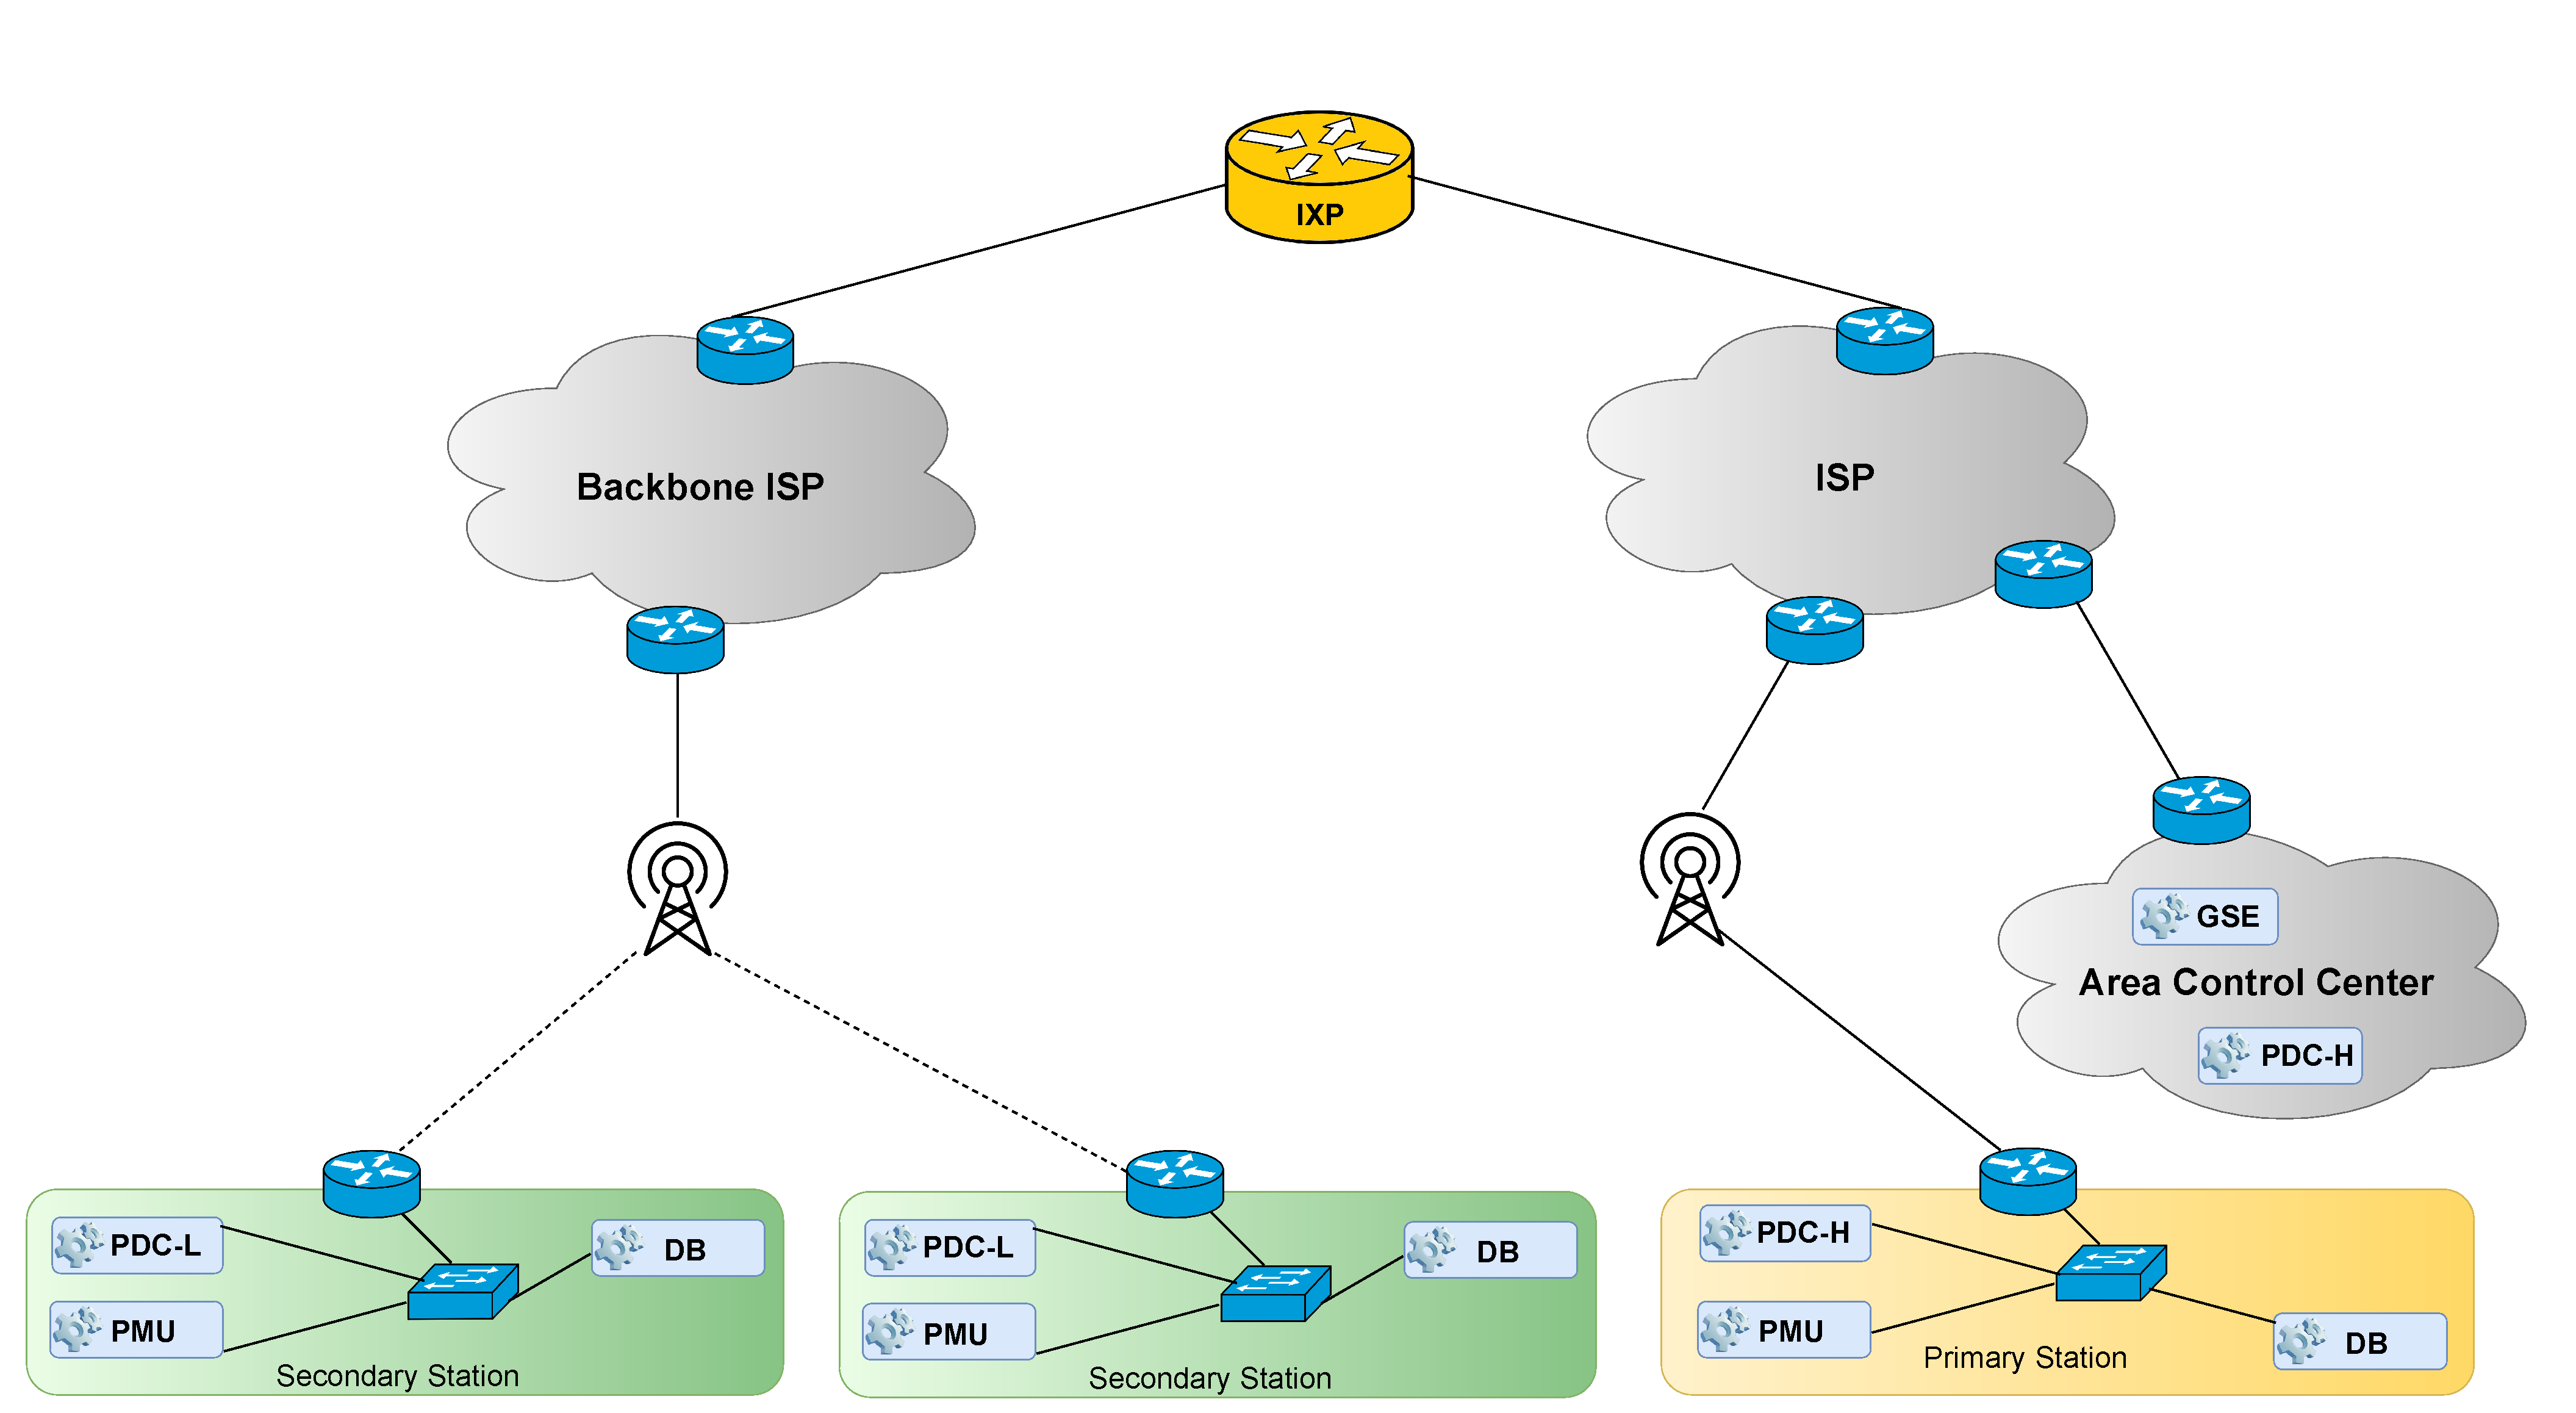
\includegraphics[scale=0.17]{Pictures/state-of-art}
\caption{Smart Grid abstract informatic model}\label{fig:art-state}
\end{figure}

\subsection{Area Control Center}
A computing node within the context of the Smart Grid that serves as an Operational Distribution Center, housing the control and management logic for the entire network.

This node is primarily responsible for overseeing the high-level PDC, where data streams from other high-level PDCs situated at primary stations are aggregated. Additionally, it manages the GSE application, which utilizes data from the aforementioned PDC to control the network.

\subsection{Station}
In the context of the Smart Grid, it is a computing node that represents an energy production or distribution station.

Primary stations typically utilize a high-level PDC to aggregate data streams from their subnet of secondary stations. Additionally, they may manage a certain number of PMUs (Phasor Measurement Units).

Secondary stations primarily handle PMUs or aggregate data streams generated by them through low-level PDCs.

\subsection{Phasor Measurement Units}
PMUs provide measurements of fundamental electrical quantities, such as voltage and current, in the form of phasors, including information on the amplitude and phase of the measured quantities. 

These measurements, synchronized via GPS and sampled at a frequency of 50 samples per second, enable precise monitoring of rapid changes in the electrical system caused by the dynamism of distributed energy resources.

PMUs offer a detailed perspective of system dynamics, overcoming the limitations of more traditional Remote Terminal Units (RTUs), which have an update period of several seconds and are not synchronized. The use of PMUs is expected to enhance the observability and reliability of the distribution system.

\subsection{Phasor Data Concentrator}
A phasor data concentrator (PDC) is designed to receive streaming synchrophasor data from phasor measurement units (PMUs) installed on power transmission lines and align these data using GPS timestamps (i.e., it "concentrates" the data based on time). 

The output of a PDC is a time-synchronized data set that is forwarded to one or more software applications.

openPDC is a flexible platform for high-speed time-series data processing, both in real-time and historically. It does not have significant computational power requirements, so it can be installed anywhere within the synchrophasor infrastructure, including on fanless computers located in substations.

\subsection{Grid State Estimation}
State estimation is a technique that allows for the reconstruction of network states, such as nodal voltages, based on available measurements and the electrical network model. Unlike traditional meters, PMU measurements, which include the phase relative to an absolute reference, simplify the state estimation problem by making it a linear system and significantly reducing the computational load. 

The objectives of state estimation include the recognition and reduction of measurement errors, the identification of topology errors, the estimation of unmeasured network quantities, and the determination of network parameters through redundant measurements.

\section{Multi-master station architecture}
Recent research has progressed towards managing individual locations such as stations within the Smart Grid using a multi-master architecture \cite{a2-1}\cite{a2-2}. This approach leverages enhanced resilience, allowing the system to withstand the failure of a master node. However, it comes with the trade-off of requiring additional resources for replicated control-plane components.

Within the cluster, application configurations (such as those for a PDC if the cluster represents a station) are stored in a high-availability distributed database system. This setup facilitates rapid and automatic redeployment to another node within the cluster in case of a failure, without needing to reconfigure the application parameters.

Consequently, the clusters support autonomous local recovery from both application and node failures.

Each cluster serves as a point of edge (for managing secondary stations) or fog (for managing primary stations) computing within the Smart Grid, depending on its location. However, the overall control architecture is manually established between each pair of clusters, each of which operates as a fully independent entity.

This manual establishment of control logic between clusters exhibits limited resilience due to potential errors in configuration and vulnerability in handling failures, while also presenting challenges in scalability.

\section{Actual limitations}
While this approach of a multi-cluster kubernetes is effective for managing a single station, it proves suboptimal when applied to an entire electrical control system.

This is due to both the complexity involved in managing a large number of nodes (with stations alone numbering in the tens of thousands, whereas Kubernetes officially supports up to 5000 nodes \cite{a3-1}) and the fundamental inability to function in isolation. 

Consider the possible failures that can occur within the architecture, as shown in Figure~\ref{fig:a-failures}. Despite there being no unrecoverable failures, since it functions as a single large Kubernetes cluster where deployments are not concentrated in one location and therefore continue to operate, any part that becomes disconnected from the network will no longer be controllable. 

This is because the master nodes on the isolated network loses the necessary consensus to initiate new workloads (new pods to manage the isolated entities) and can only partially manage existing workloads (because it can't reschedule workloads if it fails).

\begin{figure}[ht]\centering
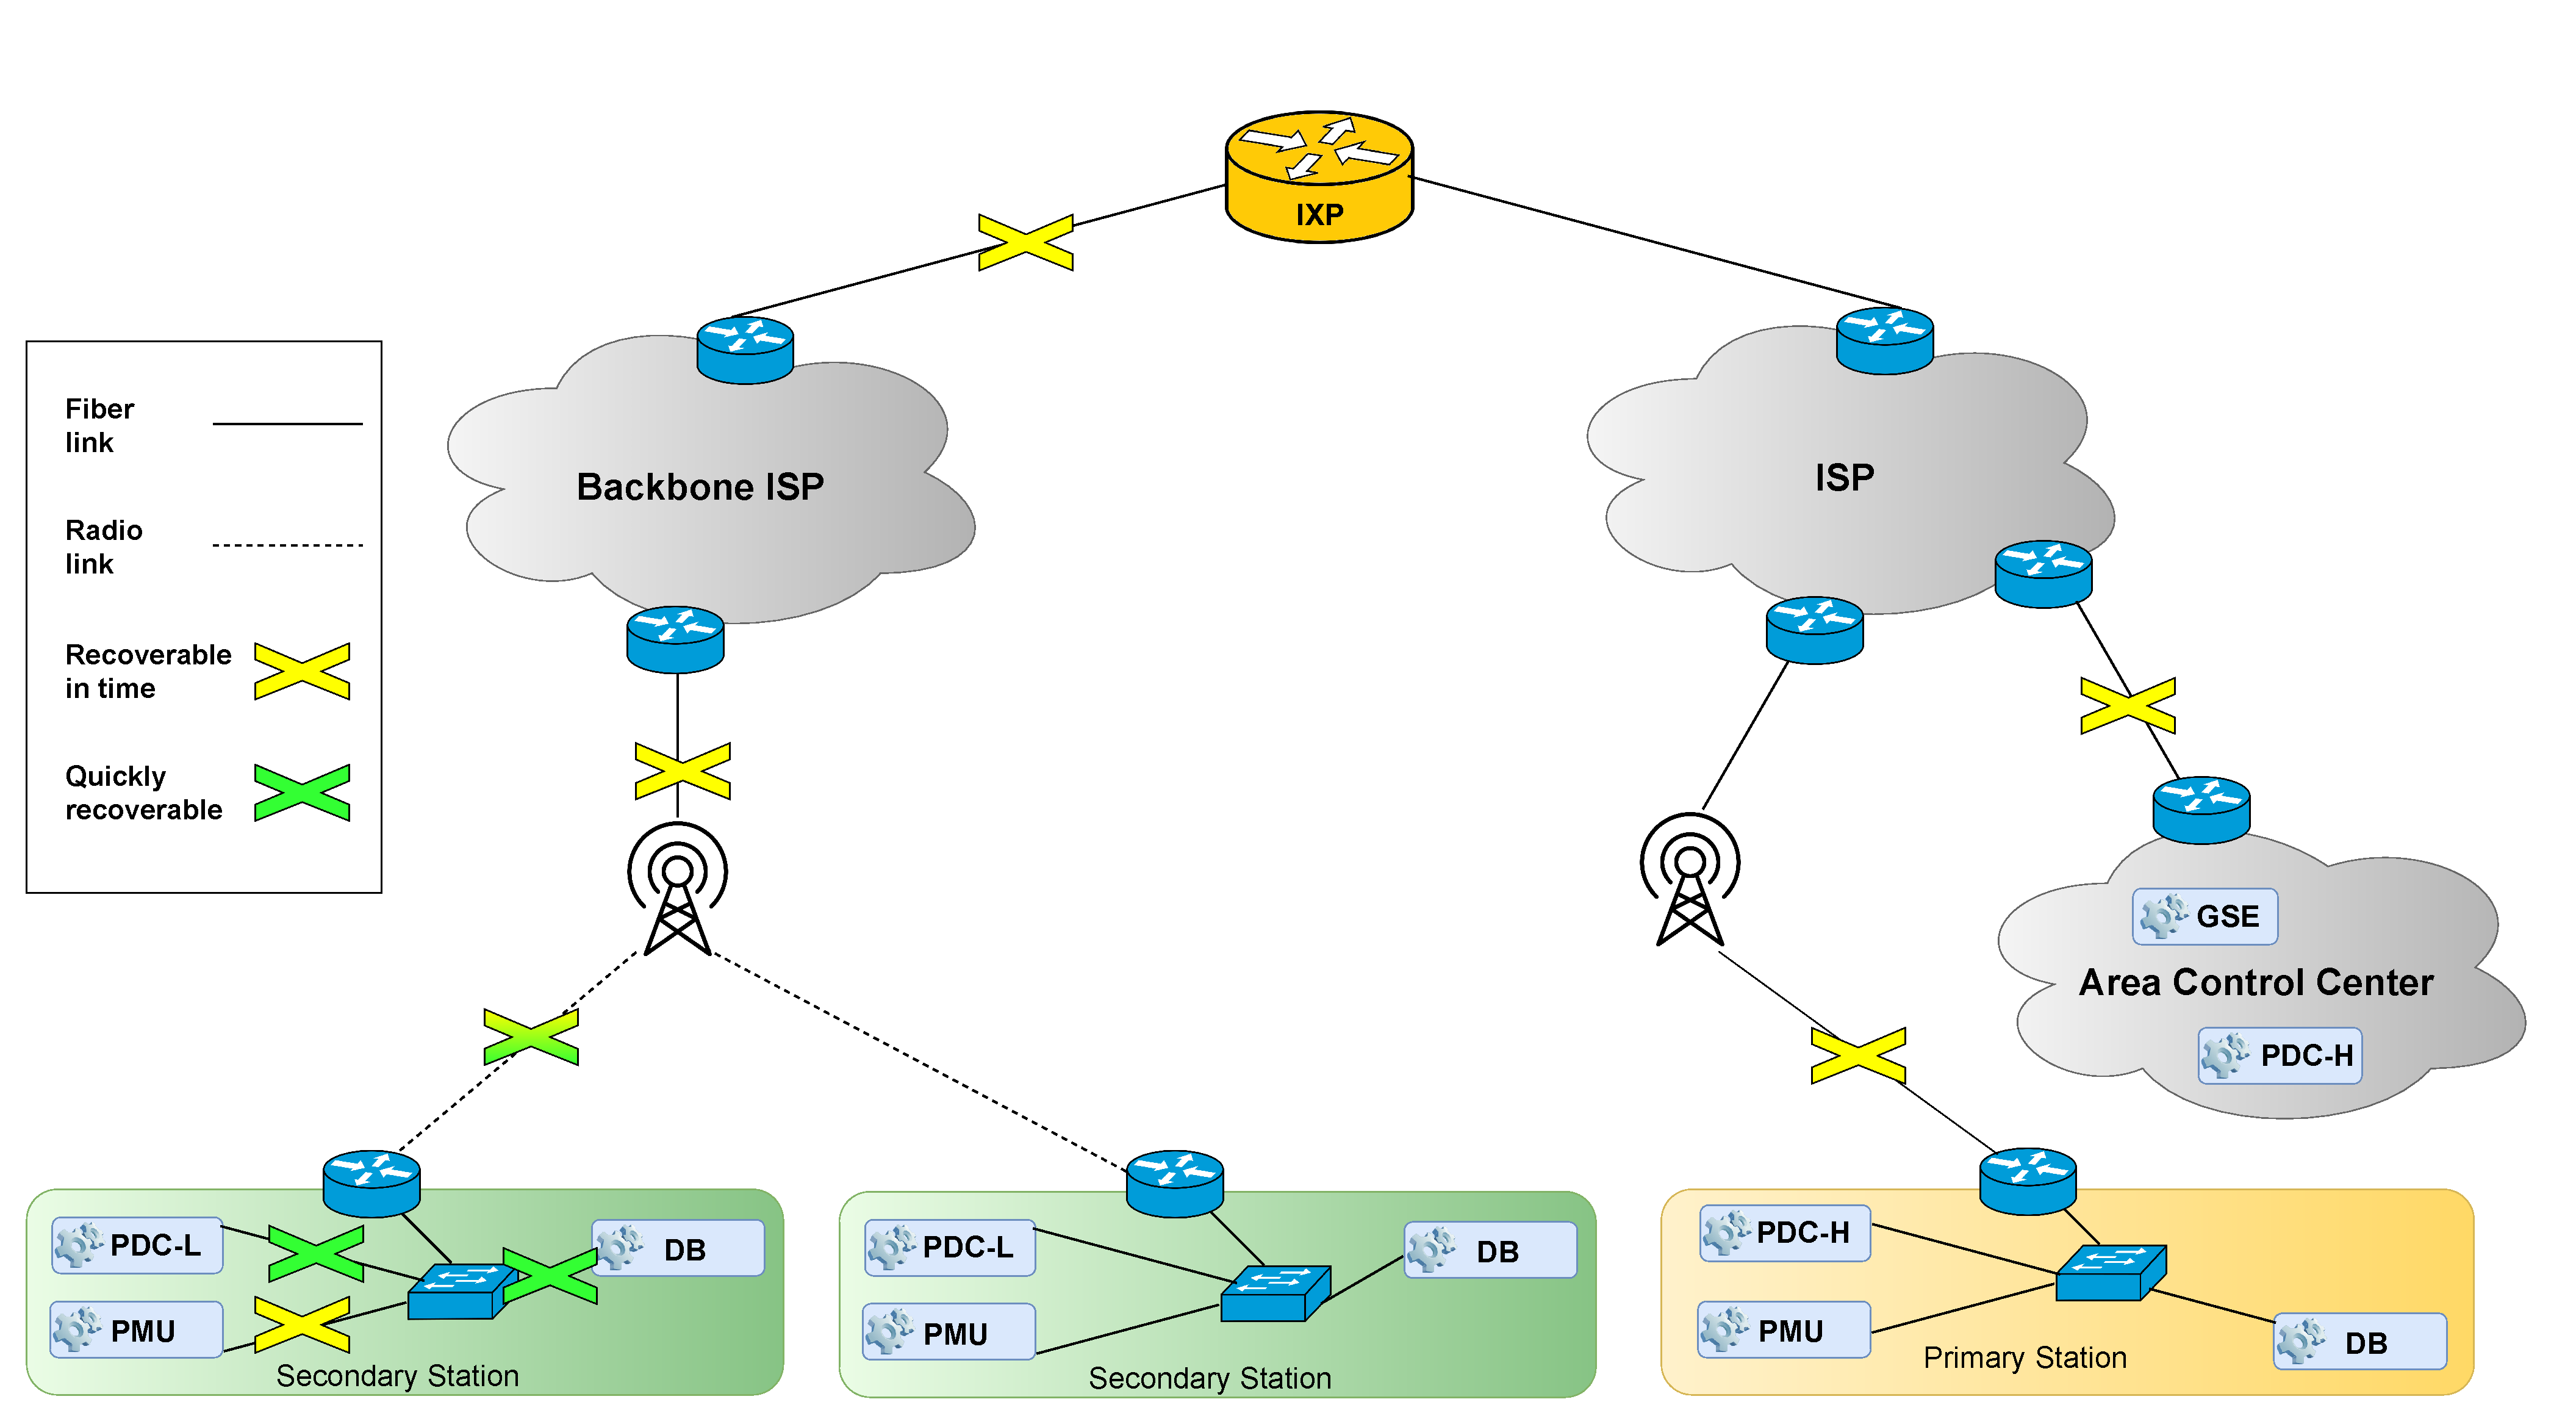
\includegraphics[scale=0.20]{Pictures/actual-failures}
\caption{Possible failures in multi-level logical domains implementation}\label{fig:a-failures}
\end{figure}

The only additional failure scenario that the translated architecture (from local environment to the entire network) can address without losing the ability to control is when an entire secondary station without source data but with the aggregator applicative becomes isolated from the network, because it simply transfer the PDC to another healty node.

However, this advantage does not outweigh the drawbacks in terms of complexity,lack of scalability, and resource demands inherent in the overall architecture. 

An additional limitation concerns the number of master nodes that must necessarily remain healthy. Considering a cluster at its maximum size (which has already been shown to be insufficient to cover an entire network), the highest resilience is achieved with 7 master nodes. In this case, the architecture continues to function as long as 4 out of the 7 master nodes remain active.

These limitations can be effectively addressed by adopting Liqo technology. For instance, instead of needing 4 nodes to remain active, only one node, the one representing the Area Control Center, needs to stay operational.

\chapter{Liqo}
Due to the rapid adoption of containers as the development environment for applications, there is now a well-established trend towards using orchestration platforms to automate the lifecycle management of containerized applications. 

Among the various implementations of these platforms, Kubernetes has gained predominant traction, to the extent that multinational corporations with dedicated cloud departments (such as Google, Amazon, Microsoft, Alibaba...) have developed proprietary solutions based on it. 

Recently, a trend similar to the one observed with container adoption has emerged, in which there is a growing need for a system that can automate relationships between various clusters managed by these platforms, whether in the cloud or on-premise. 

In this chapter will be summarized the Liqo project, designed to address this necessity, described by its creators \cite{l0-1} as "an open-source project that enables dynamic and seamless Kubernetes multi-cluster topologies, supporting heterogeneous on-premise, cloud, and edge infrastructures."

\section{Basic concepts}
The Liqo technology facilitates the creation of a unified virtual network across diverse clusters, enabling the execution of application pods on remote clusters as if they were local. This system is founded on four primary characteristics: network fabric, peering, offloading, storage fabric.

\subsection{Network fabric}
The network fabric is the subsystem of Liqo that seamlessly extends the Kubernetes networking model across multiple independent clusters, enabling pods on different clusters to communicate smoothly even when address NAT is applied.

The control plane of this subsystem resides in the network manager, instantiated as a pod responsible for managing network parameters. It handles tasks both during cluster peering and inter-cluster communications, as example featuring an interface used by the reflection logic for IP address translation.

Interconnecting two clusters involves deploying a secure VPN tunnel using WireGuard, typically established at the end of the peering process based on negotiated parameters. This functionality is implemented by the Liqo gateway component, operating within the cluster as a privileged pod. It also manages routing tables and configures necessary NAT rules to resolve address conflicts. 

Although initialized within the cluster's network, this pod utilizes a separate network namespace and policy routing to avoid conflicts with Kubernetes' existing Container Network Interface (CNI) plugins.

Traffic from local nodes/pods directed to a remote cluster is routed through an overlay network, based on VXLAN, managed by a DaemonSet component. This component is responsible for routing entries and ensures proper handling of traffic across the VPN tunnels.

\subsection{Peering}
Standard peering is the process that establishes a unidirectional link between two different Kubernetes clusters, enabling the sharing of resources and services. Through this connection, the consumer cluster can initiate processes using resources provided by the provider cluster, but not vice versa. 

In this context, the consumer cluster initiates an outgoing peering towards the provider, which reciprocates with an incoming peering from the consumer. This linkage is not exclusive, supporting possible bidirectionality and the scenario where a cluster can act as a consumer for some peerings and as a provider for others.

The peering process unfolds through the following steps:
\begin{enumerate}
\item Authentication: Each cluster uses a pre-shared token to verify its identity, which has some permissions for Liqo-related resources and negotiations.
\item Parameter Negotiation: The two clusters exchange sets of parameters necessary for finalizing the peering, including network information such as their respective CIDRs or as the amount of resources shared by the provider. 

Some of these parameters can be modified directly or using dedicated plugins, for example is possible adjusting the available resources that the provider cluster shows to the consumer cluster.
\item Creation of the Virtual Node: Within the consumer cluster, a virtual node is created to represent the resources shared by the provider cluster. Processes instantiated using the provider cluster's resources appear to be located within this virtual node, maintaining transparency in the offloading process and adhering to standard Kubernetes practices without requiring API modifications.
\item Configuration of the Network Fabric: The two clusters configure their respective network fabrics and establish a secure VPN tunnel using the previously negotiated parameters (address remapping, endpoints, etc.).
\end{enumerate}
Each connection can be differentiated based on how Liqo's control plane traffic is managed: whether it passes through the VPN tunnel alongside pod traffic (in-band control plane peering) or uses traditional communication channels (out-of-band control plane peering). 

In the former case, it is required to expose only the Liqo VPN endpoint to the pod of the remote cluster. However, this setup requires control over both clusters to negotiate network parameters through Liqo CTL tool \cite{l1-1}, resulting in a static peering configuration that requires manual intervention for updates. 

In the latter case, while to the remote pods must be expose not only the Liqo VPN endpoint but also the Kubernetes API and Liqo authentication service endpoints (as shown in the Figure \ref{fig:out-band}), it offers the flexibility to connect clusters across different domains using a pre-shared token and enables dynamic peering, so that an automatic renegotiation of parameters occurs in response to configuration changes. 

\begin{figure}[ht]\centering
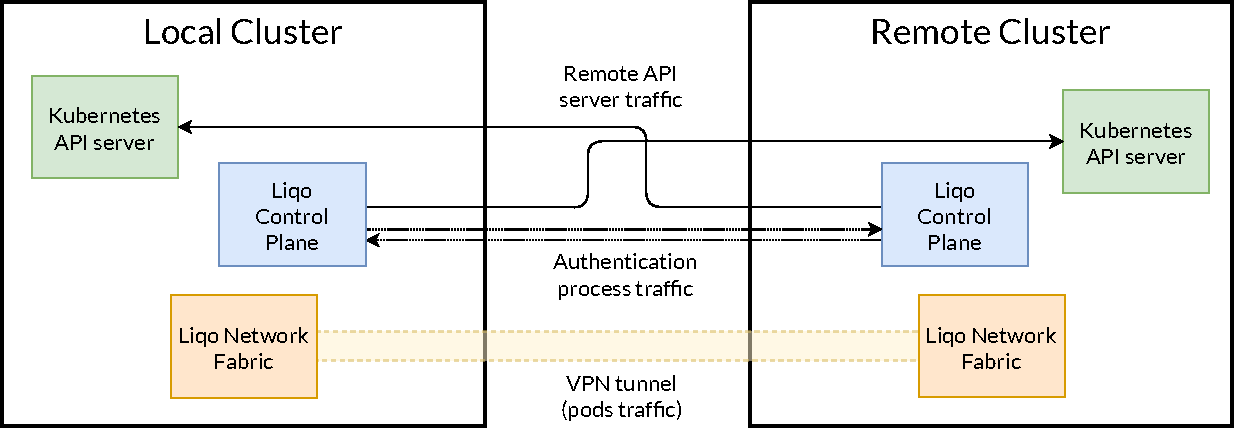
\includegraphics[scale=.5] {Pictures/out-of-band}
\caption{Out-of-band control plane peering}\label{fig:out-band}
\end{figure}

\subsection{Offloading}
Offloading is the method enabling transparent extension of the local cluster into a remote cluster, allowing Kubernetes scheduler to seamlessly schedule workloads in the remote cluster when it's deemed optimal. The virtual node is managed by an extended version of the Virtual Kubelet project, which replaces the traditional kubelet if the node isn't physical. 

In the context of Liqo, it interacts with the Kubernetes API servers of both clusters to manage artifact propagation (pods, services, config maps) and reconcile state in case of changes on the negotiated configurations. It also performs configurable periodic health checks to assess reachability of the remote API server, marking the node as unready in case of repeated failures and triggering standard Kubernetes evacuation strategies. 

An instance of the virtual kubelet is created for each remote cluster to ensure isolation and segregation of authentication tokens.

The offloading process comprises three stages:
\begin{enumerate}
\item Namespace Extension: The local cluster's namespace is extended into the remote cluster by creating a gemini counterpart namespace, which will host both offloaded pods and resources required for pod reflection.
\item Resource Reflection: Selected arctifacts from the control plane are reflected in remote clusters to ensure the operational functionality of the pods. Supported resources for reflection include service exposure (Ingress, Services, EndpointSlices), persistent storage (PersistentVolumeClaims, PersistentVolumes), and configuration data (ConfigMaps, Secrets).
\item Pod Offloading: After the scheduler schedules a pod on the virtual node, the corresponding virtual kubelet creates a mirrored pod object in the remote cluster. This object is managed by the custom resource ShadowPod~\cite{l1-2}, serving as a representation of the pod to maintain service functionality even if connectivity with the remote cluster is lost.
\end{enumerate}
Both stateless and stateful pods are supported, with the latter utilizing either the storage fabric or relying on an external volume provider.

\subsection{Storage fabric}
The storage fabric is the Liqo subsystem responsible for managing the creation of remote volumes for stateful applications. Its operation revolves around delaying the binding of a volume to a pod until it has been scheduled to a node, ensuring volumes are always created where their associated pod is scheduled. 

Subsequent scheduling adheres to a data gravity principle, transparently rescheduling the pod to the node where the physical volume resides. These behaviors are implemented through Liqo's virtual storage class, utilizing reflection mechanisms when pods are scheduled on virtual nodes to create the mirrored PVCs in remote clusters. Alternatively, it relies on the real storage class when pods are scheduled on local physical nodes.

\section{Distributed DB interaction}
At present, most of the distributed database systems doesn't support general multi-cluster architecture, primarily due to their reliance on internal headless services for direct pod-to-pod communication. These services return the IP address of the corresponding pod directly when queried, using their DNS entry, unlike regular services that route requests via kube-proxy. 

Liqo employs an address remapping mechanism to facilitate seamless communication between clusters; however, this approach results in incorrect IP resolutions for pods scheduled on remote clusters when queried by headless services.

To enable the use of these architectures, Liqo developers currently recommend\cite{l2-1} leveraging the peering process, which exposes the address ranges of the two clusters in two different ways:
\begin{enumerate}
\item Connecting a cluster to all others via peering while forcing a pod of the distributed system onto it: This approach ensures that the service in that cluster is aware of all real address ranges, allowing replication through the forced pod, which becomes a critical point.
\item Creating a full mesh of peering between various clusters: This ensures that each headless service knows the addresses of all others, and this is the solution adopted in this research.
\end{enumerate}
Some distributed database architectures, such as those implemented by the Percona XtraDB Cluster Operator, may introduce additional complexity. After receiving the translated IP of a remote pod, they may encounter difficulties establishing a connection, primarily because their cluster logic operates with standard Kubernetes component independently of Liqo. This requires the implementation of distinct CIDRs across clusters, ensuring that traffic is routed through Liqo components to establish connections correctly.

\chapter{General topology Partial Mesh Star}\label{chap:partial-mesh-star}
In this chapter will be described the process that led to the selection of the partial mesh star architecture, a model capable of applying the logical paradigms of edge/fog computing to a multi-cluster architecture while ensuring the possibility of deploying high-availability systems. Initially, the structural choices will be discussed, based on both the multi-cluster environment and the requirements of the adopted technologies (Percona, Liqo, etc.).

Potential use cases will then be described, demonstrating the flexibility of the logical hierarchical architectures that can be implemented. Finally, we will evaluate the characteristics and various limitations that this model entails.

\section{Physical/net architecture}
The first step was to consider how to abstract a logical model from the initial real-world situation. The electric power control and monitoring network, as shown in the figure \ref{fig:real-net}, can be schematized using both hierarchical tree topology graphs and peer-to-peer topology graphs.

\begin{figure}[ht]\centering
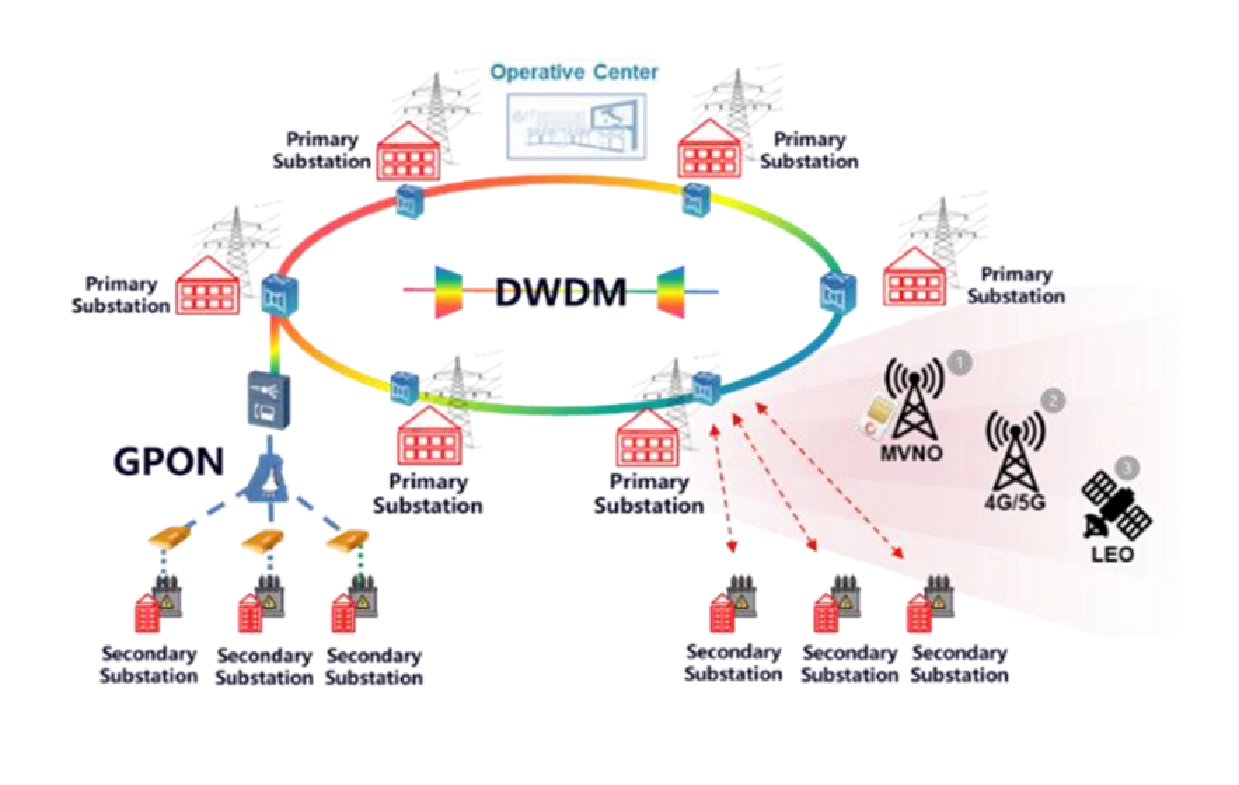
\includegraphics[scale=0.6]{Pictures/real-scheme-net}
\caption{Target Telecommunications Architecture Foreseen in the 2023 Development Plan for e-distribution}\label{fig:real-net}
\end{figure}


Peer-to-peer should be discarded because, although the nodes representing the stations can be both data providers and receivers, the node representing the Area Control Center needs to exercise centralized control over all other nodes. Additionally, not all nodes have sufficient processing capabilities, especially if they represent secondary stations.

Among the various tree topology models, the star model is the only one that can be physically implemented using the standard version of Liqo. Indeed, it does not allow the offloading of an already offloaded namespace to prevent critical situations such as circular offloading. This means that all multi-level hierarchical topologies cannot be physically implemented without making customized changes to the technology's code. Moreover, distributed HA database systems tend to need to be in a single namespace, and multi-namespace solutions via operators do not support multi-cluster technologies as they cannot know the namespaces of other clusters.

The partial mesh version of the star model, which allows direct connections between leaves, is necessary for the correct transparent multi-cluster functioning of distributed database systems that rely on headless services. Each cluster that uses the same database system will need, in addition to having the offloaded namespace of the database, a direct connection with all other clusters, thus creating a partial mesh topology (partial because the connections do not necessarily have to be bidirectional).

\section{Logic complex hierarchy using labels and affinity}
A simple partial-mesh star topology offers only a two-level physical separation: a central node and the leaves. It lacks the necessary flexibility to manage the various real-world scenarios encountered in a monitoring and distribution network. Therefore, it is necessary to introduce a strategy to construct a complex logical topology on the existing physical model. This strategy is based on the use of Kubernetes' native label and affinity mechanisms.

Each cluster will be identified by a group of labels that specify its position in the desired logical topology and can be used by the scheduler to distribute the workload according to the intended logic. The node affinity mechanism can be used both to distinguish between different clusters and to differentiate the various nodes within a cluster, as it allows specifying different labels as targets. This way, one can define the label that identifies the cluster as well as the labels of the individual nodes within the cluster.

Pod affinity, on the other hand, is used to enforce coexistence conditions between pods on the same node. These mechanisms also offer a degree of flexibility, as they provide both "required" and "preferred" options. The "preferred" option allows the scheduler to prioritize the specified target for pod placement while still considering alternative targets if the preferred one is unavailable.

The following subsections will discuss some basic logical topologies, from which one can start to build their desired configuration.

\subsection{Independent Groups}\label{sec:indipendent-groups}
The leaf clusters of the partial-mesh star model are segmented into independent groups by assigning each node within the cluster a label that uniquely identifies its respective group. This method establishes distinct logical areas, as peering between clusters is only necessary within the same group (and only in case of using a distributed database system), to which separated workloads can be allocated. To enhance the delineation of these divisions, the root node could assign a separate namespace to each group, thereby also increasing security between them.

These groups are not mutually exclusive, provided there is no logical contradiction among the identifying labels. Consequently, a cluster may simultaneously belong to multiple groups, as demonstrated by leaf C in Figure \ref{fig:group-ind}.

\begin{figure}[ht]\centering
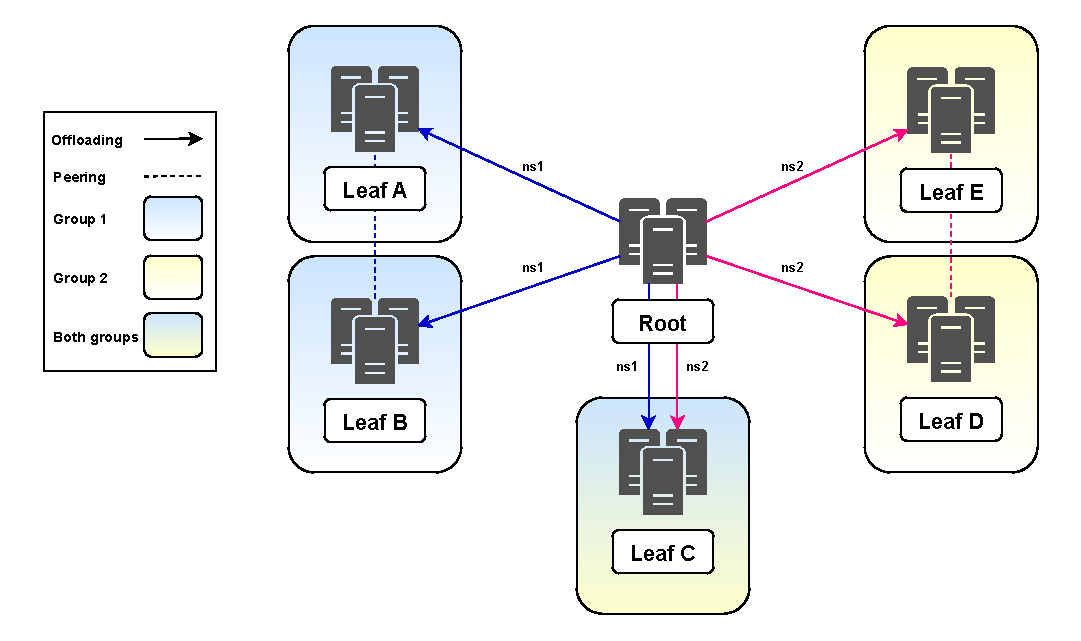
\includegraphics[scale=0.7]{Pictures/Group-v6}
\caption{Independent Groups Scheme}\label{fig:group-ind}
\end{figure}

\subsection{Dependent Groups}
The leaf clusters of the partial-mesh star model are divided following a logical hierarchy by assigning a label indicating their position within the hierarchy. This approach creates dependent logical areas, as peering is necessary even between clusters belonging to different groups if a distributed database system is used. Figure \ref{fig:group-dep} illustrates the worst-case scenario, where the database domain encompasses all leaf clusters. This topology supports new behaviors, such as allowing not only the selection of which groups to schedule workloads within the same domain.

This mechanism allows for the creation of multiple logical hierarchies within the same physical network, each with its own set of labels. Within a given logical hierarchical structure, a cluster can belong to only one group. However, when considering multiple structures, a cluster can belong to different groups.

\begin{figure}[ht]\centering
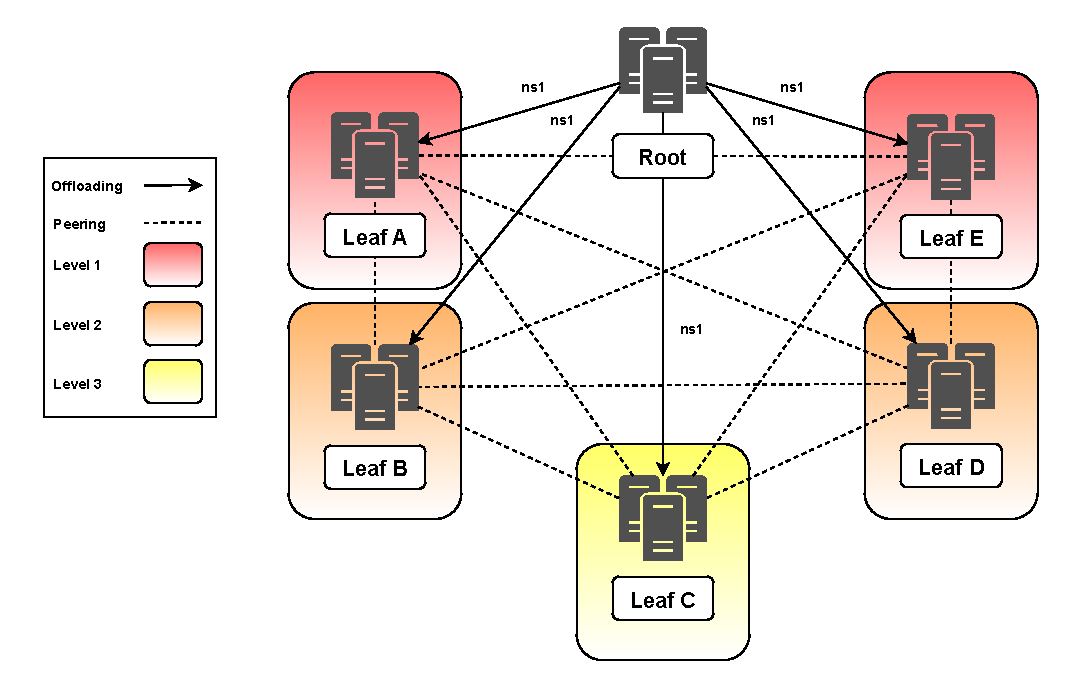
\includegraphics[scale=0.7]{Pictures/Level-v4}
\caption{Dependent Groups Scheme}\label{fig:group-dep}
\end{figure}

\section{Partial Mesh Star Analysis}
As previously illustrated, the partial mesh star topology allows for the use of systems not originally designed for multi-cluster environments, such as distributed HA databases. However, this feature results in a quadratic increase in the number of peerings required between clusters within the database domain. This is because it requires at least a unidirectional peering full mesh. The number of links can be determined using the formula \eqref{eq:eq-link-mesh}:
\begin{equation} \label{eq:eq-link-mesh}
\text{Link} = \frac{N(N-1)}{2}
\end{equation}
where N is the number of clusters.

The increase in the number of peerings only affects the time needed to set up the entire architecture during its creation, as the consumption of additional resources is negligible (CITA PAPER Marco?).

The label mechanism offers substantial flexibility in selecting the logical architecture to overlay on the physical infrastructure. However, a drawback is the linear increase in setup time as the number of clusters expands. This characteristic renders the partial mesh star topology ideal for systems with relatively stable physical topologies, facilitating quick adjustments in logical configurations. While significant logical topological changes are supported, they require a corresponding setup time.


\chapter{Possible implementations}
This chapter will discuss the potential implementations of the partial mesh star topology within the context of a computer network dedicated to energy monitoring. The network primarily consists of the Area Control Center, primary stations, and secondary stations, each managed by its own Kubernetes cluster.

\section{Logical domains}
This implementation is depicted in Figure~\ref{fig:domains}, where the Area Control Center occupies the central position in the star topology, establishing unidirectional peering with offloading to every other entity in the topology, whether it is a primary station or a secondary station.

\begin{figure}[ht]\centering
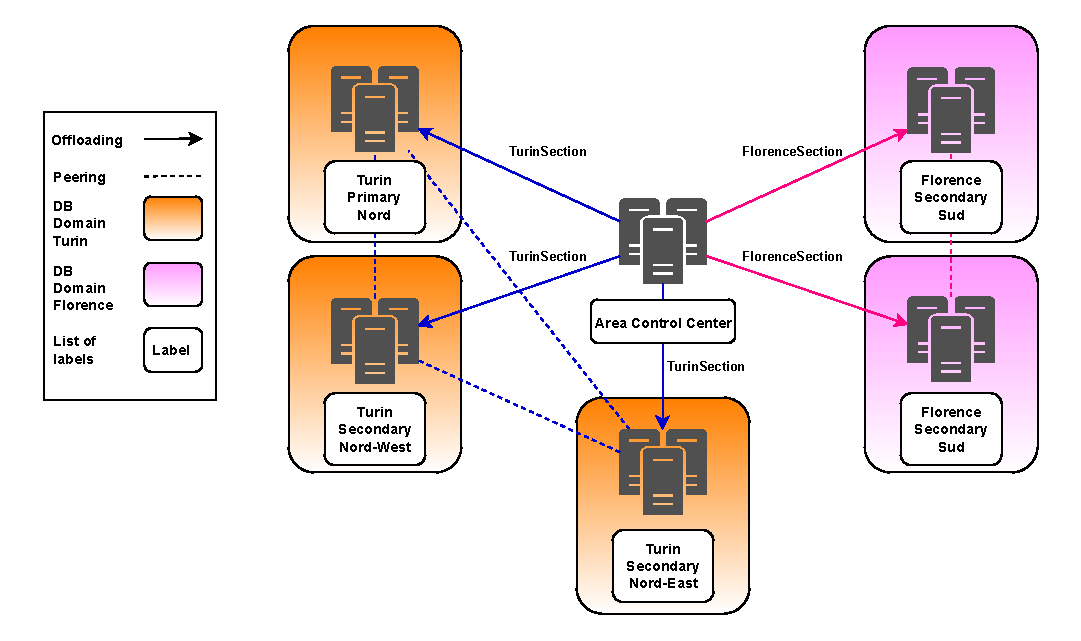
\includegraphics[scale=0.7]{Pictures/Domain-v3}
\caption{Logical domains scheme.}\label{fig:domains}
\end{figure}

This allows the Area Control Center to manage all application deployments without the need to delegate them to other nodes.
The remaining clusters are divided into groups, typically consisting of a primary station and its associated secondary stations. These groups represent a logical domain of applications with their own high-availability distributed database system and, therefore, do not have interconnections among them. Within a group, the clusters form a full mesh of unidirectional peerings for the database system's operation, and they share the same offloaded namespace from the Area Control Center. 


\subsection{Logical domains analysis}

This architecture allows for the highest degree of resilience, as considering every possible failure in the control and power distribution network infrastructure, represented in Figure~\ref{fig:failures}, the only fault that is not automatically recoverable is the disconnection of the Area Control Center.

\begin{figure}[ht]\centering
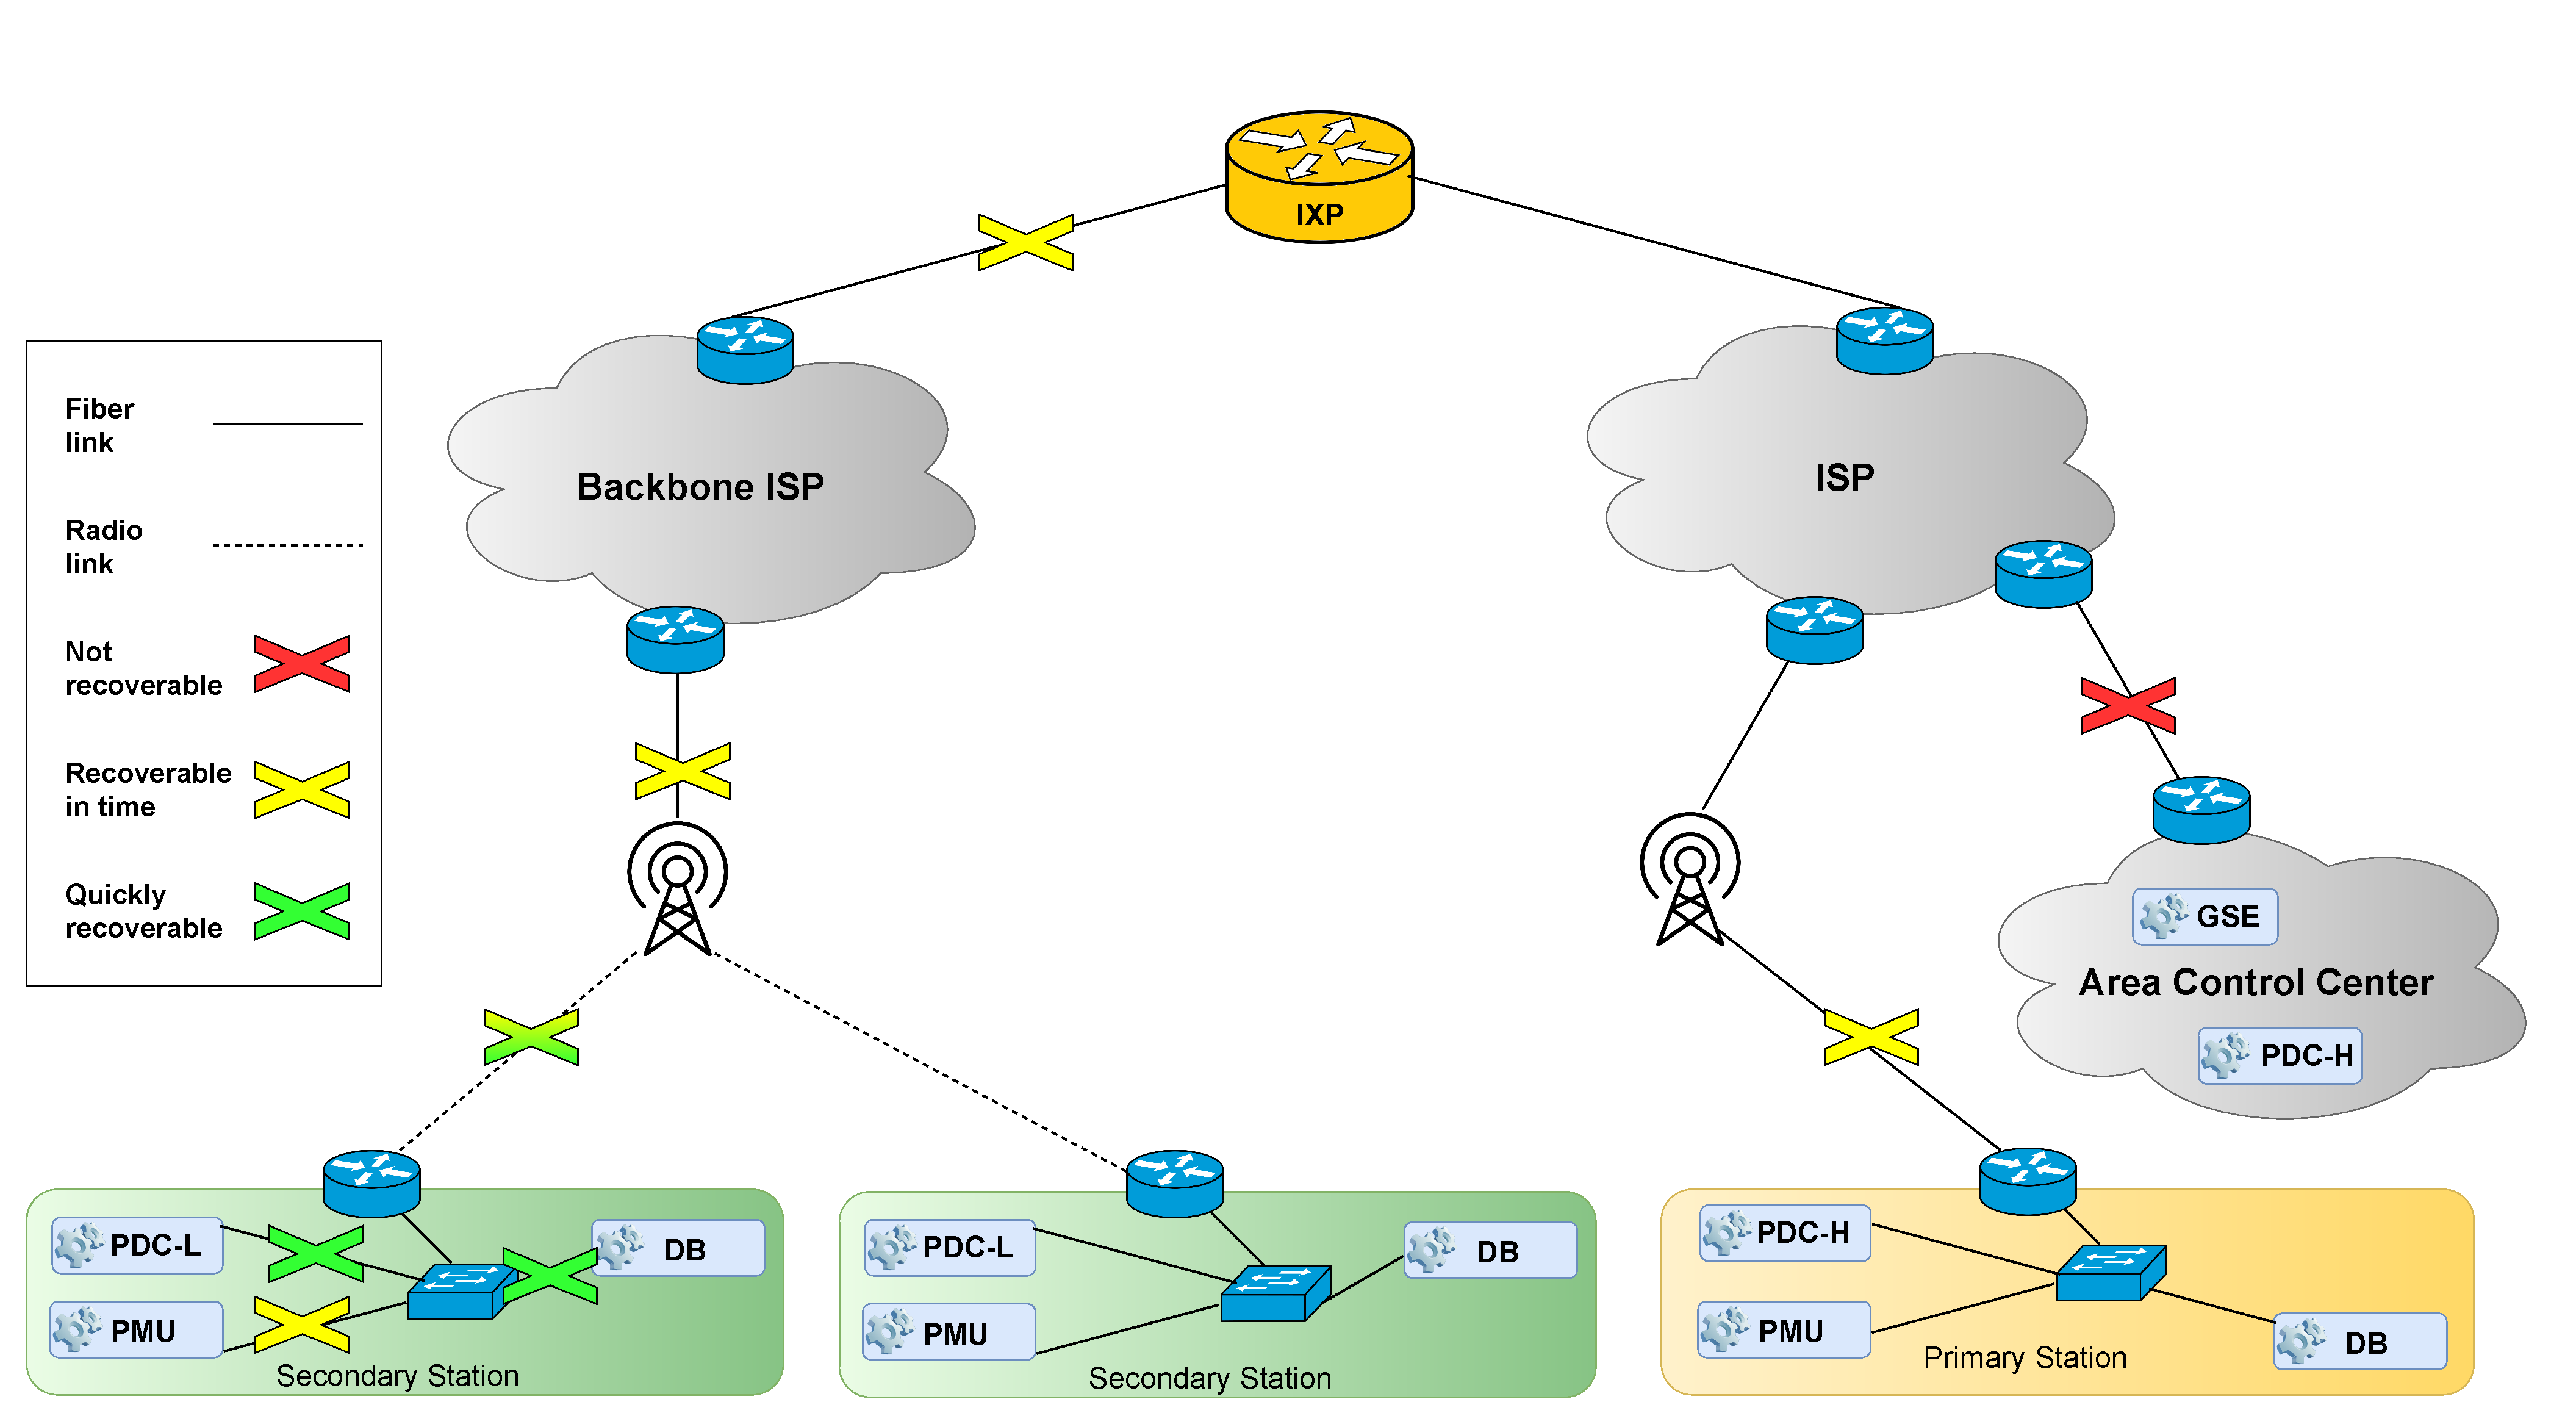
\includegraphics[scale=0.20]{Pictures/failures}
\caption{Possible failures in logical domains implementation.}\label{fig:failures}
\end{figure}

The cluster representing the Area Control Center is a critical point as it hosts the central logic of the network, but the effects of a failure or disconnection of this node are negligible when compared to environmental constraints:

\begin{enumerate}
\item In the event of a physical failure of the central node, deployments would be lost, making the reconciliation process with the entire network impossible. However, this is negligible because without the central node's logic, the network would not be observable by default.
\item In the event of a complete disconnection from the network, active workloads would continue to function, but the reconciliation process for stateful applications (as the database system) will not occur since, by the point of view of the deployments, there would not be enough surviving replicas to maintain the system. Yet, this is also negligible as it falls under the same scenario as before.
\end{enumerate}

In contrast, all other failures are recoverable from the perspective of the Area Control Center. Failures within a cluster are generally recoverable in a short time as the applications are automatically and quickly ricreated into a healthy node (which can belong to either the local cluster or a remote cluster) in case of disconnection or internal pod failure. 

Disconnections of nodes, entire clusters, or parts of the network containing data production sources (PMUs) are automatically recoverable only with the restoration of the connection itself, as the PMU is physical hardware tied to its node and cannot be moved to others.

The aforementioned concerns the perspective of the Area Control Center, but as described in the previous chapter, the disconnected part of the network continues to function perfectly, and thanks to Liqo technology, additional applications can be instantiated to support the temporary independence of the network.

The continuation of operations can be observed in Figure~\ref{fig:stream}, which illustrates the data stream about frequency values seen by an instance of PDC lower and its directly superior PDC higher, shortly before and shortly after the disconnection of the cluster hosting the PDC lower and its data sources, which occurred at 44,633 s. PDC lower continues to receive data from the sources, operating in an isolated environment, while PDC higher stops receiving the data stream from the isolated source. 

\begin{figure}[ht]\centering
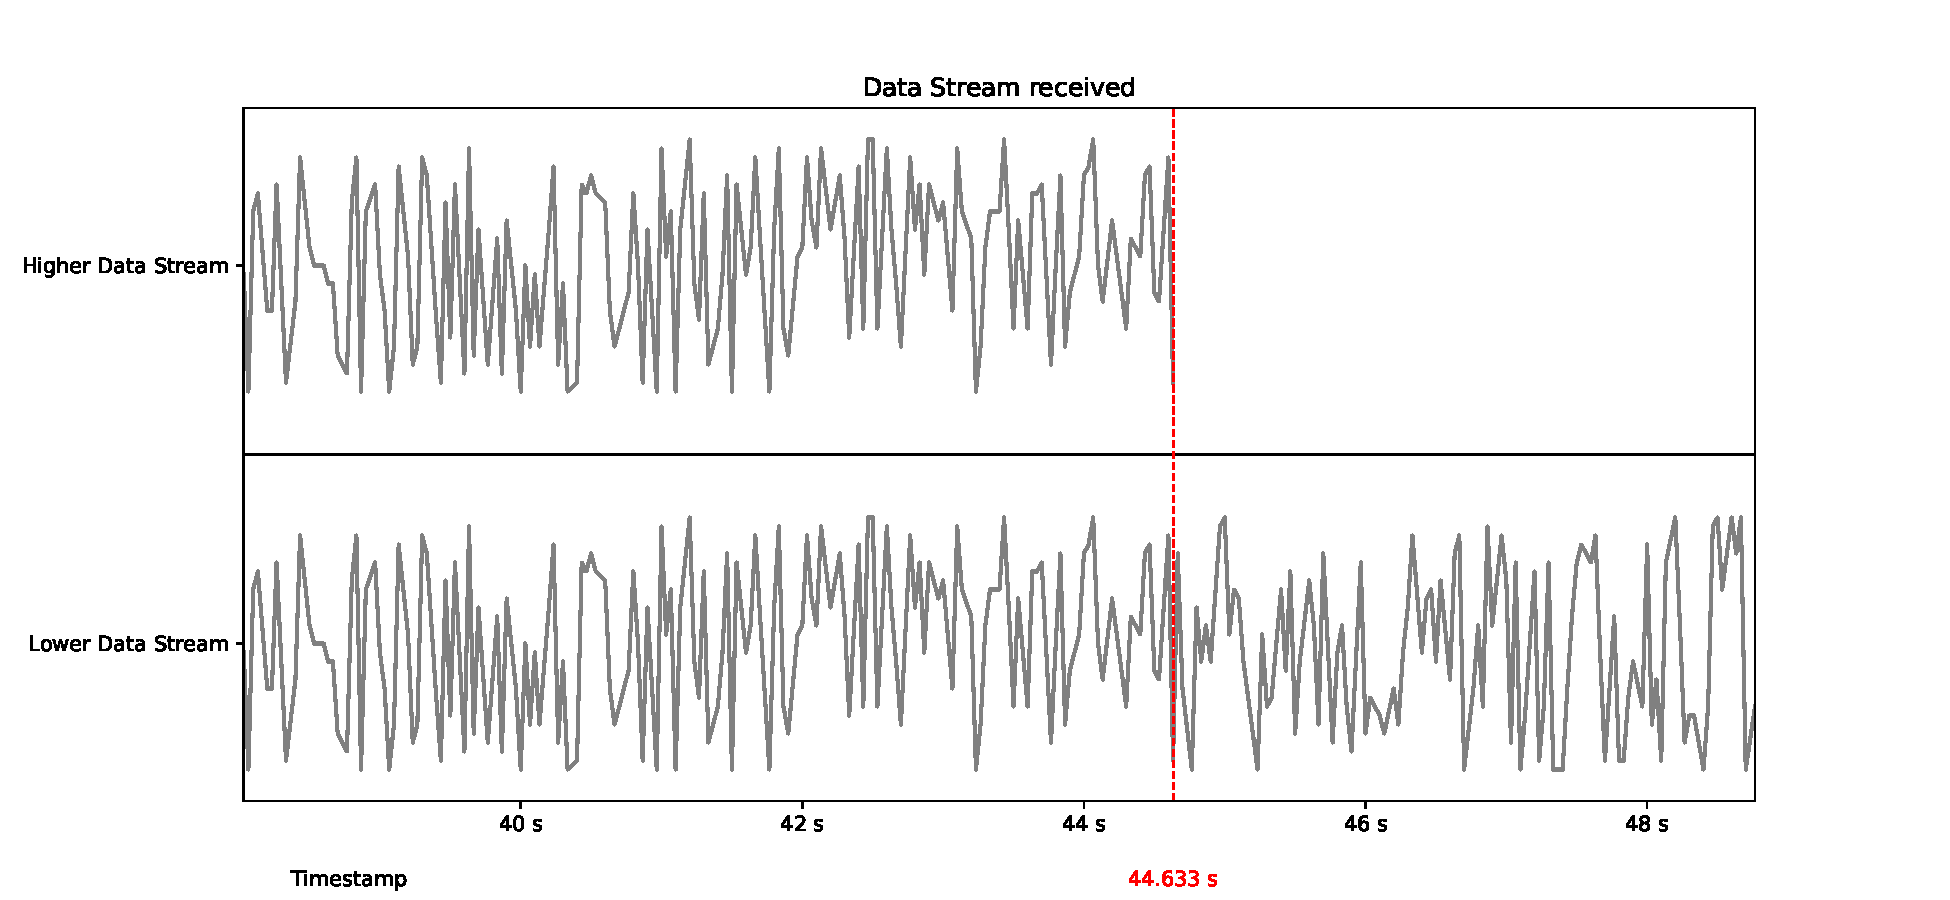
\includegraphics[scale=0.5]{Pictures/data-stream}
\caption{Data Stream comparison in case of failure.}\label{fig:stream}
\end{figure}

Comparing the risks arising from the failure of one component with those that an extended local solution encompassed, as shown in Table ~\ref{t:6}, it can be noted that many have decreased, as there is no longer the possibility of the network remaining unobservable. The risks related to PMU failures have remained the same, as it cannot be rescheduled to another node.

\begin{table}[ht]              
\centering 
\begin{tabularx}{\textwidth}{|l|c|X|}
\hline
\textbf{Component Failure} & \textbf{Severity} & \textbf{Cause}\\ 
\hline
\raisebox{-0.75cm}{Single PMU} & \raisebox{-0.75cm}{Low-> Low} & Generally the number of other PMUs guarantees the observability threshold. \\
\hline
\raisebox{-0.75cm}{Multiple PMUs} & \raisebox{-0.75cm}{Low-High-> Low-High} & It depends on whether the number of other PMUs guarantees the observability threshold.\\
\hline
\raisebox{-0.75cm}{Single PDC-l} & \raisebox{-0.75cm}{Moderate-High-> Low-Moderate} & The observability of the network is impaired until the PDC is rescheduled onto another node.\\
\hline
\raisebox{-0.75cm}{Multiple PDCs-l} & \raisebox{-0.75cm}{Moderate-High-> Low-Moderate} & The observability of the network is impaired until the PDCs are rescheduled onto another nodes. \\
\hline
\raisebox{-0.75cm}{Single PDC-h} & \raisebox{-0.75cm}{High-> Moderate}& The observability of the network is impaired until the PDC is rescheduled onto another node. \\
\hline
\end{tabularx}
\caption[Component failures on Logical Domains topology overview.]{Component failures on Logical Domains topology overview.} \label{t:6}  
\end{table}

The limitations of this architecture pertain to scalability, as each cluster requires its own distinct CIDR for the transparent operation of high-availability distributed database systems. Additionally, each peering creates a virtual representative node in the central cluster, limiting the number of possible clusters to 5000, according to the official Kubernetes documentation.

\section{Multi-level logical domains}
The implementation described in this section leverages a star topology twice, once with a partial mesh version and once with a full version, as shown in Figure~\ref{fig:level-imp}. This follows the division of stations into primary and secondary, although it could be adapted to n subdivisions.

\begin{figure}[ht]\centering
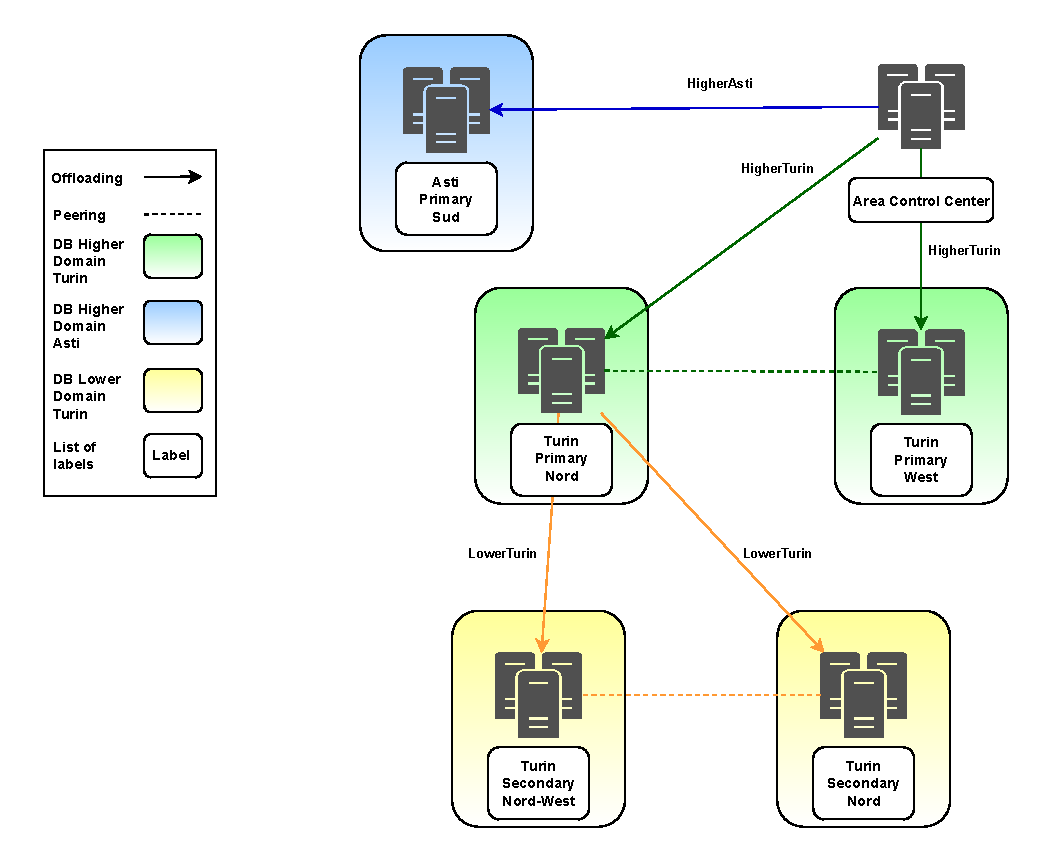
\includegraphics[scale=0.7]{Pictures/2level}
\caption{2 Level logical domains.}\label{fig:level-imp}
\end{figure}

The first topology used is a partial mesh star topology used to connect the Area Control Center (central cluster) with all primary stations (leaf clusters). The central cluster handles the deployment of high-level applications along with their respective distributed database systems, offloading the corresponding namespace through peering to the respective group of primary stations.

The groups of primary stations are composed of a main primary station, where workload is preferably directed (using labels), while the others in the group primarily serve as backups in case of failure of the main station. This means that primary stations can be in multiple groups, one where they are primary and others where they function as backups, leveraging the topology seen in Chapter~\ref{chap:partial-mesh-star} section~\ref{sec:indipendent-groups}.

The main primary station of each group also serves as the central cluster in the second star topology, connecting not only to the backup primary stations but also to all secondary stations under its jurisdiction. In our implementation, this will be a full mesh star topology, but a partial mesh could also be used if the secondary stations do not share the same distributed database system.

In this second topology, the main primary station handles the deployment of low-level applications along with their respective high-availability distributed databases, consequently offloading the namespace to its secondary stations. The data stream for monitoring, which passes through two different namespaces (from the low-level to the high-level), relies on external exposure services such as load balancers and ingress, enabling access to the high-level application whether it resides in the primary station or, due to a failure, in one of the backup primary stations.


\subsection{Multi-level Logical domains analysis}

This architecture enhances scalability limits compared to the previous implementation by reducing the number of peerings managed by the Area Control Center,  as shown in Figure~\ref{fig:failures2}, and by requiring distinct CIDRs only within the secondary topologies associated with a primary station, allowing for reuse across different types.

\begin{figure}[ht]\centering
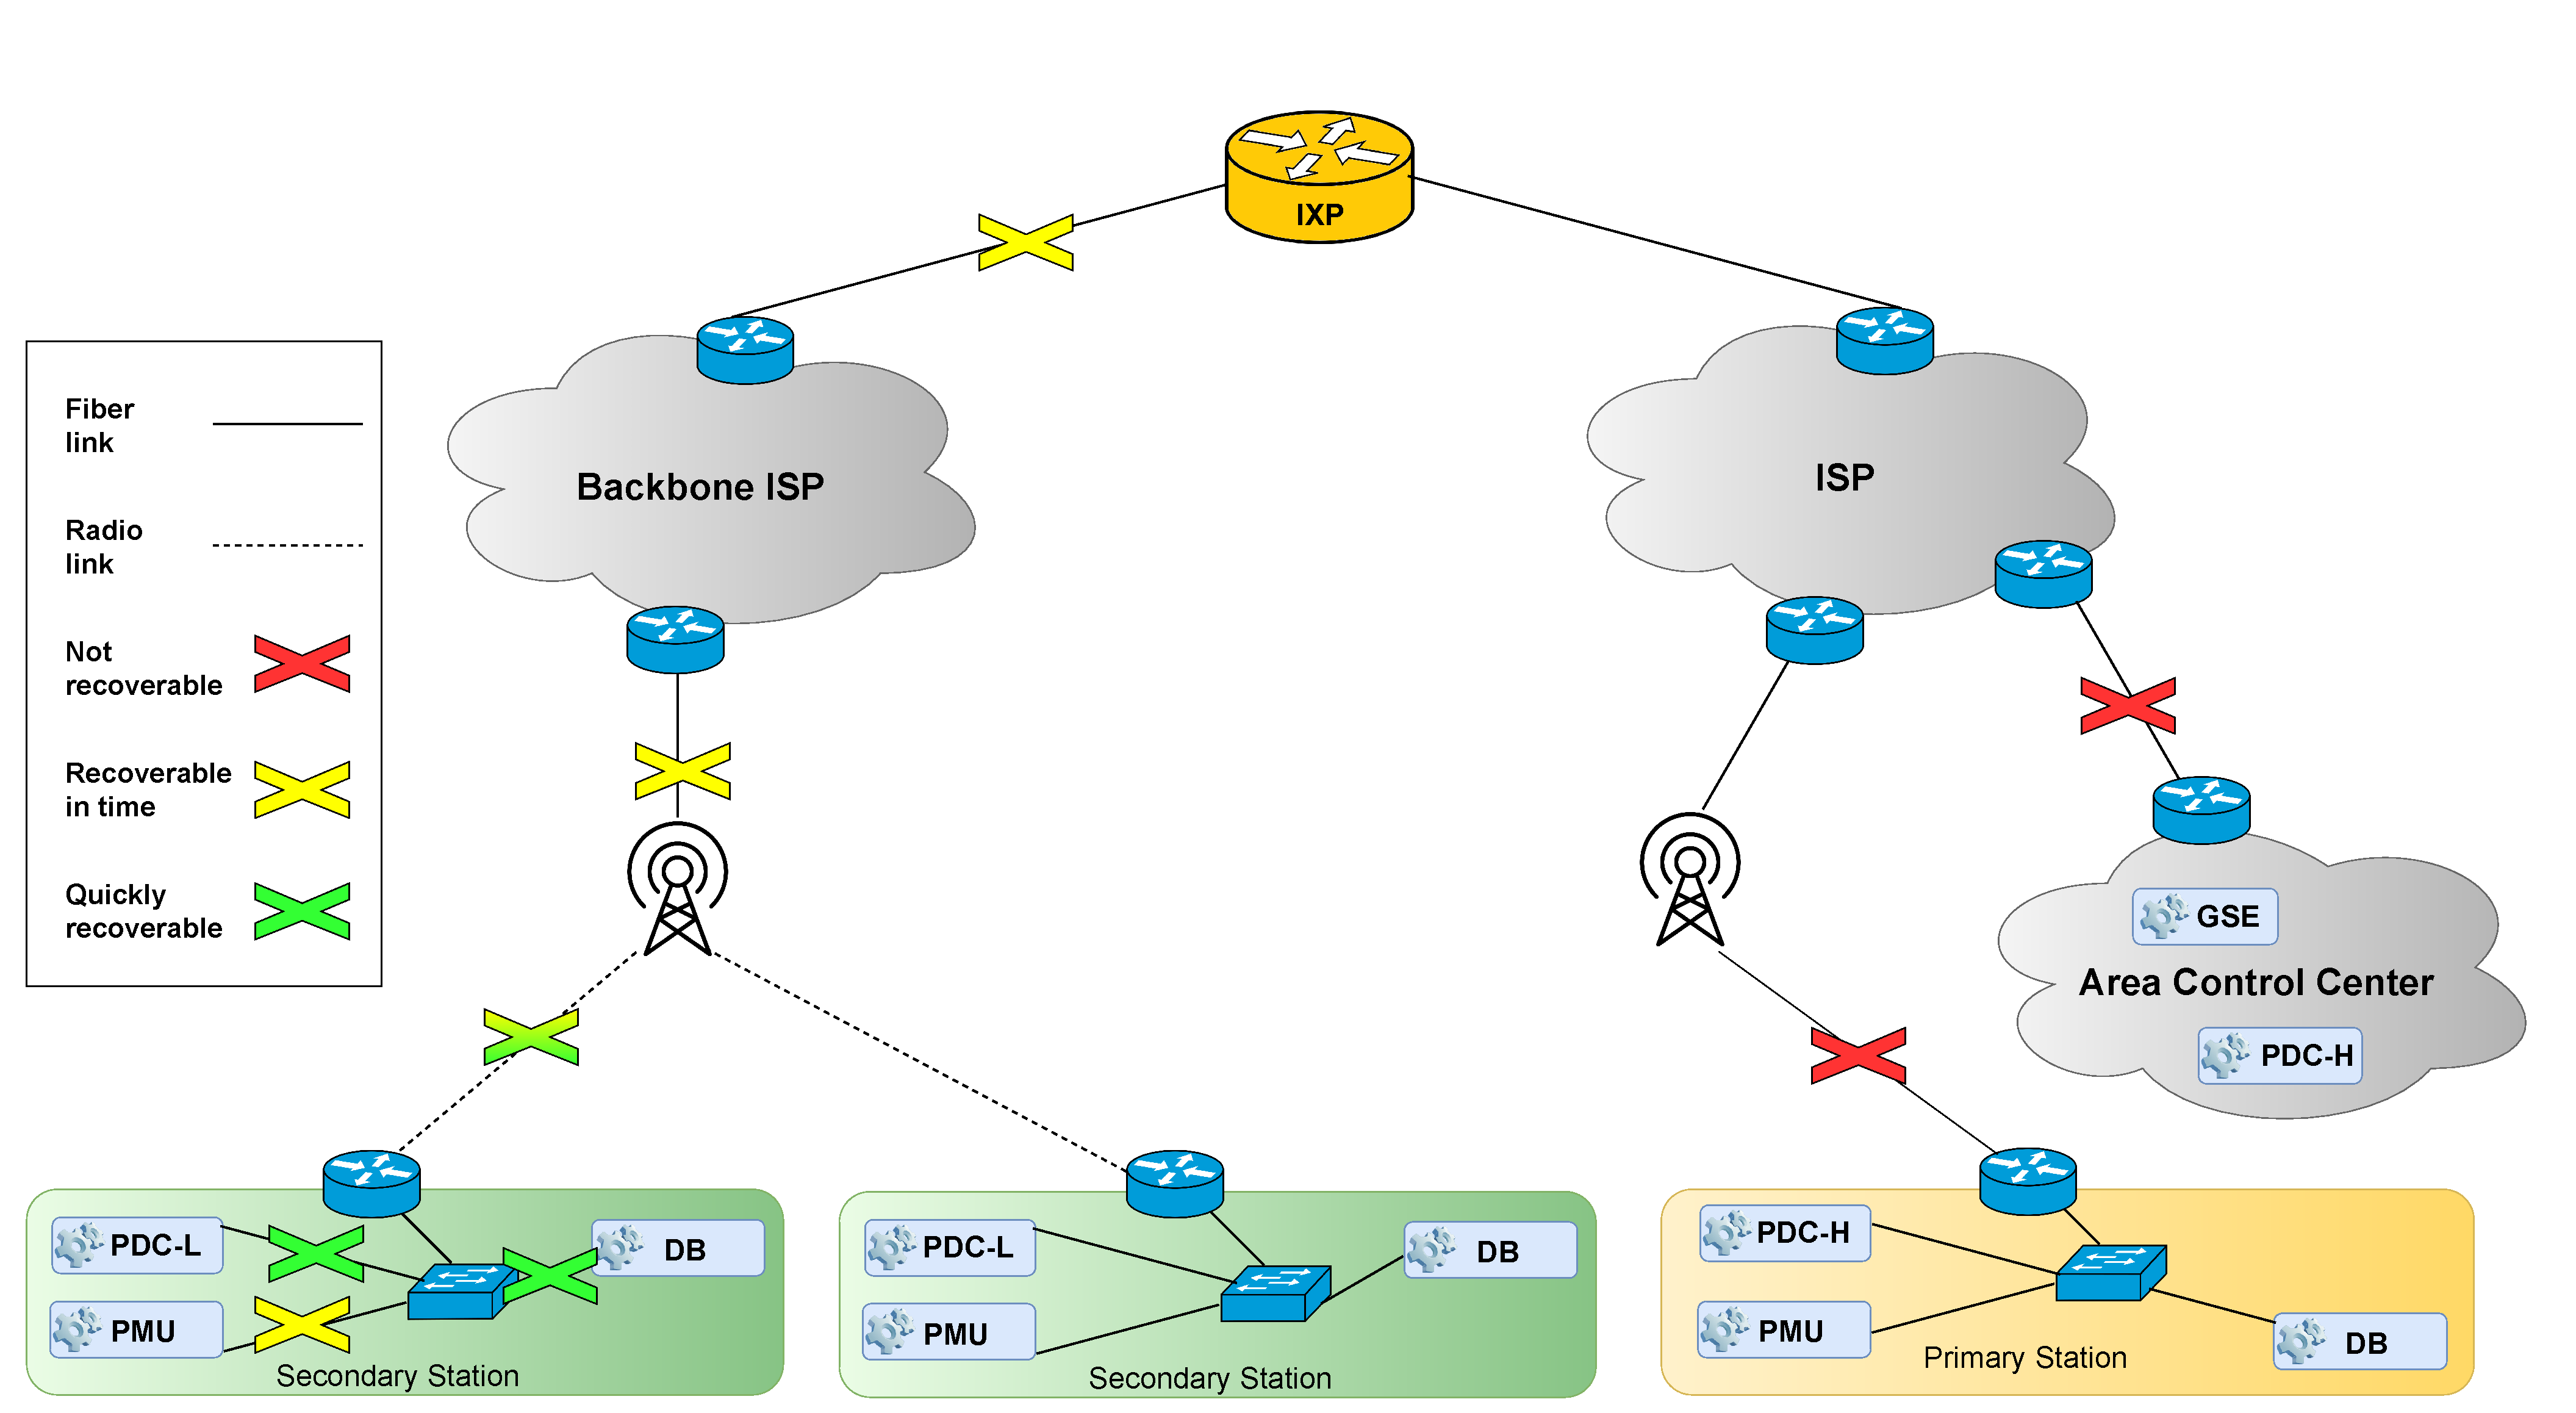
\includegraphics[scale=0.20]{Pictures/failures2}
\caption{Possible failures in multi-level logical domains implementation.}\label{fig:failures2}
\end{figure}

However, this benefit is balanced by a decrease in overall resilience, because in addition to the critical point represented by the Area Control Center, all primary stations that manage a subnetwork of secondary stations also become critical points. This is because a failure or disconnection of the primary station results in the loss of deployment for low-level applications, which is not a feature supported by Liqo technology, thus necessitating a system reset upon reconnection.

Comparing the risks arising from the failure of one component with those that an extended local solution encompassed, as shown in Table ~\ref{t:7}, it can be noted that many have decreased, as there is no longer the possibility of the network remaining unobservable. The risks related to PMU failures have remained the same, as it cannot be rescheduled to another node.

\begin{table}[t]              
\centering 
\begin{tabularx}{\textwidth}{|l|c|X|}
\hline
\textbf{Component Failure} & \textbf{Severity} & \textbf{Cause}\\ 
\hline
\raisebox{-0.75cm}{Single PMU} & \raisebox{-0.75cm}{Low-> Low} & Generally the number of other PMUs guarantees the observability threshold. \\
\hline
\raisebox{-0.75cm}{Multiple PMUs} & \raisebox{-0.75cm}{Low-High-> Low-High} & It depends on whether the number of other PMUs guarantees the observability threshold.\\
\hline
\raisebox{-0.75cm}{Single PDC-l} & \raisebox{-0.75cm}{Moderate-High-> Low-Moderate} & The observability of the network is impaired until the PDC is rescheduled onto another node.\\
\hline
\raisebox{-0.75cm}{Multiple PDCs-l} & \raisebox{-0.75cm}{Moderate-High-> Low-Moderate} & The observability of the network is impaired until the PDCs are rescheduled onto another nodes. \\
\hline
\raisebox{-0.75cm}{Single PDC-h} & \raisebox{-0.75cm}{High-> Moderate}& The observability of the network is impaired until the PDC is rescheduled onto another node. \\
\hline
\end{tabularx}
\caption[Component failures on Multi- level Logical Domains topology overview.]{Component failures on Multi-level Logical Domains topology overview.} \label{t:7}  
\end{table}

This thesis focuses on achieving the highest degree of resilience; therefore, the following chapter will focus on testing the first implementation, as there is no risk of having to redeploy the software components in a subnetwork of secondary substations in the event of a failure of the entire associated primary station cluster.

It is important to note that these two implementations are not mutually exclusive; they can be implemented simultaneously within the same physical network, in cases where different parts of the network require varying degrees of resilience.

\chapter{Domain peering evaluation}
In this chapter, we present the analyses conducted on the logical domain grouping implementation, chosen for its higher resilience compared to the multi-level implementation.

\section{Test Environment}
The test environment was created by leveraging the functionalities of Crownlabs, an open-source platform associated with the Politecnico di Torino, which was developed during the years of the Coronavirus spread.

\subsection{Crownlabs}
Crownlabs is an open-source project created to provide students with access to laboratory systems and services during the challenging times of the coronavirus pandemic, which imposed severe travel restrictions. In fact, the name derives from the virus itself and its initial purpose, as "Crown" translates to "Corona" in Italian and labs measn laboratories.

The authors of this project were a group of volunteers primarily composed of MSc students who, within just a few weeks of very hard work, as described on the project website~\cite{e1-1}, managed to deliver a functioning version, to address the university places closures mandated by the Italian government.

Nowadays, Crownlabs continues to be supported by students, and its functionalities have expanded: it not only allows the remote use of laboratory machines through a web browser, enabling both personal exercises and group work, but also leverages the Politecnico di Torino's data center to instantiate and use virtual machines transparently within an internal network.

It is precisely this latter functionality that has been utilized, as the Kubernetes clusters used were composed of these virtual machines.

\subsection{Nodes configuration}
Each virtual machine representing a node in a cluster possesses the following characteristics, chosen to simulate low computational capacity typical of devices found in energy monitoring and distribution stations.
\begin{itemize}
\item \textbf{Operating system:}  Ubuntu server 20.04 LTS.
\item \textbf{CPU:} 4 core.
\item \textbf{RAM:} 8 GB.
\item \textbf{Disk memory:} 25 GB.
\end{itemize}

\subsection{Software configuration}
Di seguito vengono specificate le versioni delle piattaforme utilizzate:
\begin{itemize}
\item \textbf{K3s:} v1.24.17+k3s1.
\item \textbf{Liqoctl:} v0.10.2.
\item \textbf{Liqo:}  v0.10.2.
\item \textbf{PDC:}  v2.4.
\item \textbf{Database:} Percona XtraDB operator v1.11.0.
\item \textbf{Database connector:} MYSQL connector v8.2.
\end{itemize}

It should be noted that certain parameters of the k3s kubelet and manager controller have been adjusted to decrease the cluster response time in case of failure, as detailed in the Table~\ref{t:1}. In contrast, the virtual kubelet instantiated by Liqo has not undergone any changes.

\begin{table}[ht]              
\centering 
\begin{tabularx}{\textwidth}{|l|c|X|}
\hline 
\textbf{Option} &\textbf{Value} &\textbf{Description} \\
\hline
\raisebox{-0.25cm}{node-status-update-frequency} & \raisebox{-0.25cm}{10s -> 5s} & Specifies how often kubelet posts node status \\
\hline
\raisebox{-1.5cm}{node-monitor-grace-period} & \raisebox{-1.5cm}{40s -> 20s} & Specifies the amount of time in seconds that the Kubernetes Controller Manager waits for an update from a kubelet before marking the node unhealthy. Must be N times more than kubelet's nodeStatusUpdateFrequency, where N means number of retries allowed for kubelet to post node status \\
\hline
\raisebox{-0.5cm}{pod-eviction-timeout} & \raisebox{-0.5cm}{300s -> 5s}&This parameter specifies how long Kubernetes waits before evicting pod from a node marked as "NotReady" \\
\hline
\end{tabularx}
\caption[Kubelet and Controller Manager list of parameter changes]{Kubelet and Controller Manager list of parameter changes} \label{t:1}  
\end{table}

\subsection{Cluster configuration}
Due to the limit of 5 virtual machines, the system was organized into 5 Kubernetes clusters, each comprising a single node. As shown in Figure~\ref{fig:test}, the topology is a fully-meshed star topology where the root cluster occupies the central position, hosting all deployments of the PMU, PDC, and database applications. Through Liqo peering, it offloads the test namespace to the leaf clusters.

The leaf clusters are connected by unidirectional peering for the transparent operation of the distributed Percona database system, and they will be the only locations where the pods of the aforementioned applications can be scheduled.

\begin{figure}[ht]\centering
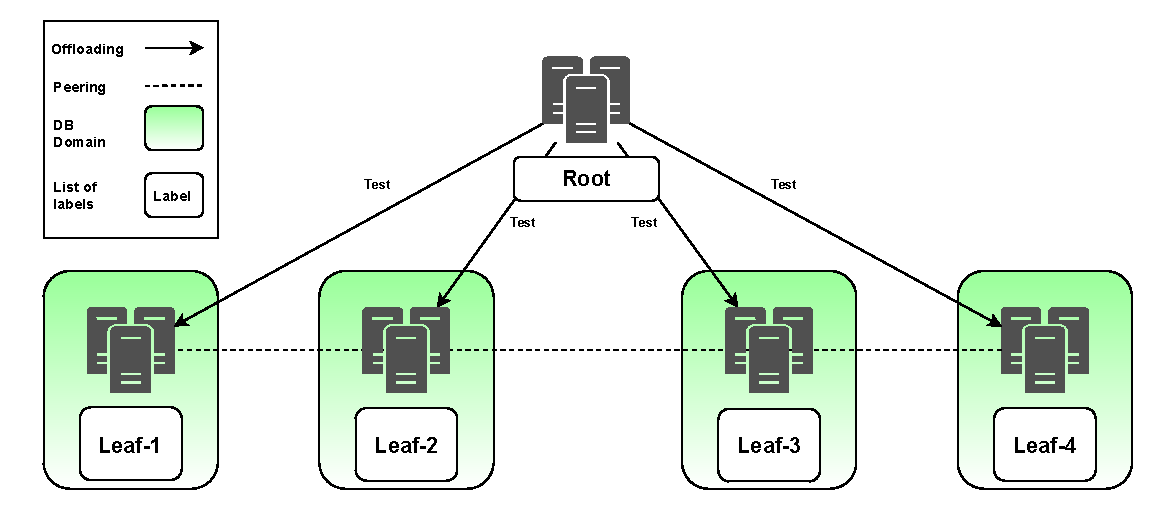
\includegraphics[scale=0.5]{Pictures/test}
\caption{Configuration test environment}\label{fig:test}
\end{figure}

\section{Latency}
In this section, the latency increase due to the overhead generated by Liqo technology will be evaluated using 4 virtual machines. One machine is consistently used as the secondary member (Root), while the others represent the primary member (Leaves).

The maximum tolerated data communication latency for state estimation applications is approximately 1000 ms.

Typically, data, as depicted in Figure~\ref{fig:latency}, traverses about 4 clusters. The first two clusters usually consist of secondary stations, the third is the primary station overseeing the subnetwork of the two secondary stations, and the fourth is the Area Control Center containing the applications utilizing the data.

\begin{figure}[ht]\centering
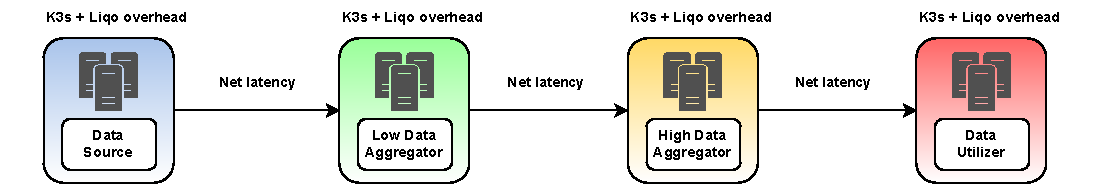
\includegraphics[scale=0.7]{Pictures/latency-schema}
\caption{Data flow from source to destination}\label{fig:latency}
\end{figure}

Therefore, the overall latency derives from the sum of Kubernetes + Liqo overhead for each individual cluster, plus the latencies of the networks connecting these clusters.

The networks connecting these clusters typically consist of optical fiber networks for links between primary stations and Area Control Centers, and either fiber optic or radio links for the subnetwork of secondary stations. According to the 2023 Development Plan of e-distribution~\cite{e2-1}, these networks include fiber optic cables illuminated with DWDM technology for connecting primaries to the control center, GPON fiber architectures, or 5G/LTE/4G radio links for connections between secondary and primary stations.

Let's consider the New AT/MT transformation station "Livigno" (SO) as presented in the 2023 development plan of e-distribution~\cite{e2-2}, as it represents an extreme case regarding the extension of the managed territory, approximately 400 km$^2$ in a rural environment. To estimate the network latency, we consider a fairly central location of the station within the area, hence the maximum distance between it and the secondary substations can be hypothesized to be about 200-300 km. Over this distance, we consider a worst-case scenario of a 4G LTE network based on radio links, with cell towers approximately 10 km apart.

The network latency is calculated by adding the propagation speed over 300 km and the signal processing time for each cell tower. Assuming a signal processing time of about 20 ms and a propagation speed of 1 ms, the total latency would be 20 * 30 + 1 = 601 ms. For the distance between the primary station and its respective Area Control Center, a time of 1 ms can be assumed, as this technology operates at around tens of microseconds over 140 km.

Therefore, the network latency considering one of the worst-case scenarios (use of radio links in a vast territory) can be approximated to about 601 ms, leaving a theoretical limit of 399 ms for the overhead of the technologies.

\subsection{Latency test}
Given that data in the architecture is transmitted using TCP protocols, which utilize acknowledgments (ACKs), latency is measured as the round-trip time of a packet. The tests were conducted using the ping command, with approximately 1000 iterations per test, individually executed from the Leaf machines to the Root machine.

Firstly, to establish a baseline for the tests, the network latency was calculated by averaging the mean of three ping values obtained from the virtual machines towards the root machine, as shown in the Table~\ref{t:2}.

\begin{table}[ht]              
\centering 
\begin{tabular}{|l|c|}
\hline
\textbf{Virtual machine} & \textbf{Latency}  \\ 
\hline
Leaf-1 & 0.689 $\pm$ 0.447  \\
\hline
Leaf-2 & 0.760 $\pm$ 0.771 \\
\hline
Leaf-3 & 0.715 $\pm$ 0.468 \\
\hline
Avg & 0.721 $\pm$ 0.581 \\
\hline
\end{tabular}
\caption[Network average latency ]{Network average latency} \label{t:2}  
\end{table}

After establishing the network latency, we proceed to calculate the latency between a pod located on different Leaf nodes and a pod in the Root node, where the Leaf nodes and the Root node belong to the same cluster, shown in Table~\ref{t:3}, or belong to different clusters peered with Liqo, shown in Table~\ref{t:4}.

\begin{minipage}{0.45\textwidth}
  \centering
  \vspace{0.5cm}
  \begin{tabular}{|l|c|}
  \hline
  \textbf{Cluster Node} & \textbf{Latency}  \\ 
  \hline
  Leaf-1 & 0.735 $\pm$ 0.294  \\
  \hline
  Leaf-2 & 0.992 $\pm$ 0.568 \\
  \hline
  Leaf-3 & 0.936 $\pm$ 0.483 \\
  \hline
  Avg & 0.888 $\pm$ 0.267 \\
  \hline
  \end{tabular}
  \captionof{table}{Latency between pod on different nodes, but on the same cluster}
  \label{t:3}\vspace{0.5cm}
\end{minipage}%
\hspace{0.05\textwidth} % Adjust the horizontal space between the tables
\begin{minipage}{0.45\textwidth}
  \centering
  \vspace{0.5cm}
  \begin{tabular}{|l|c|}
  \hline
  \textbf{Remote Node} & \textbf{Latency}  \\ 
  \hline
  Leaf-1 & 1.269 $\pm$ 0.724  \\
  \hline
  Leaf-2 & 1.400 $\pm$ 0.829 \\
  \hline
  Leaf-3 & 1.368 $\pm$ 0.903 \\
  \hline
  Avg & 1.346 $\pm$ 0.821 \\
  \hline
  \end{tabular}
  \captionof{table}{Latency between pod on different clusters, peered with Liqo}
  \label{t:4}\vspace{0.5cm}
\end{minipage}

The increase due to Liqo is measured by subtracting the average latency from Table~\ref{t:3}, which is the sum of network latency + Kubernetes overhead, from the average latency shown in Table~\ref{t:4}, which is the sum of network latency + Kubernetes overhead + Liqo overhead. This calculation yields the result shown in Table~\ref{t:5}. The result shows that the overhead added by Liqo is negligible compared to the total tolerated latency of 1000 ms, as well as compared to one of the worst-case scenarios such as the Livigno case.

\begin{table}[ht]              
\centering 
\begin{tabular}{|l|}
\hline
\textbf{Average Liqo Latency} \\ 
\hline
0.458  $\pm$ 0.864 ms \\
\hline
\end{tabular}
\caption{Average Liqo Latency} \label{t:5}  
\end{table}

The latency between pods on different Kubernetes clusters without multi-cluster technologies was not tested, as the goal is to demonstrate the latency increase using Liqo across different clusters compared to using a single Kubernetes cluster connecting all nodes.

\section{k3s reaction time}

In the upcoming test, two clusters of virtual machines connected via unidirectional Liqo peering were utilized: the consumer cluster and the provider cluster. The objective was to show the consumer cluster's response time in the event of disconnection of the virtual node representing the provider cluster, for any reason.

The test involved two scripts. The first script disabled the network interface on the virtual machine running Liqo in the provider cluster and recorded the timestamp. The second script executed a loop on the consumer cluster, running 'kubectl get node' every 0.4 seconds, and appending the output with a timestamp. (A shorter interval wasn't feasible due to the command execution time.)

The results are depicted in Graph~\ref{graph:k-reaction}. Comparing these results with findings from previous thesis~\cite{e3-1} about the local solution using only Kubernetes, which utilized virtual machines running on different physical machines with slightly different parameter settings, it is evident that the order of magnitude remains consistent. This indicates that the introduction of Liqo technology does not add noteworthy delays compared to the typical delays of a straightforward Kubernetes architecture.

\begin{figure}[ht]\centering
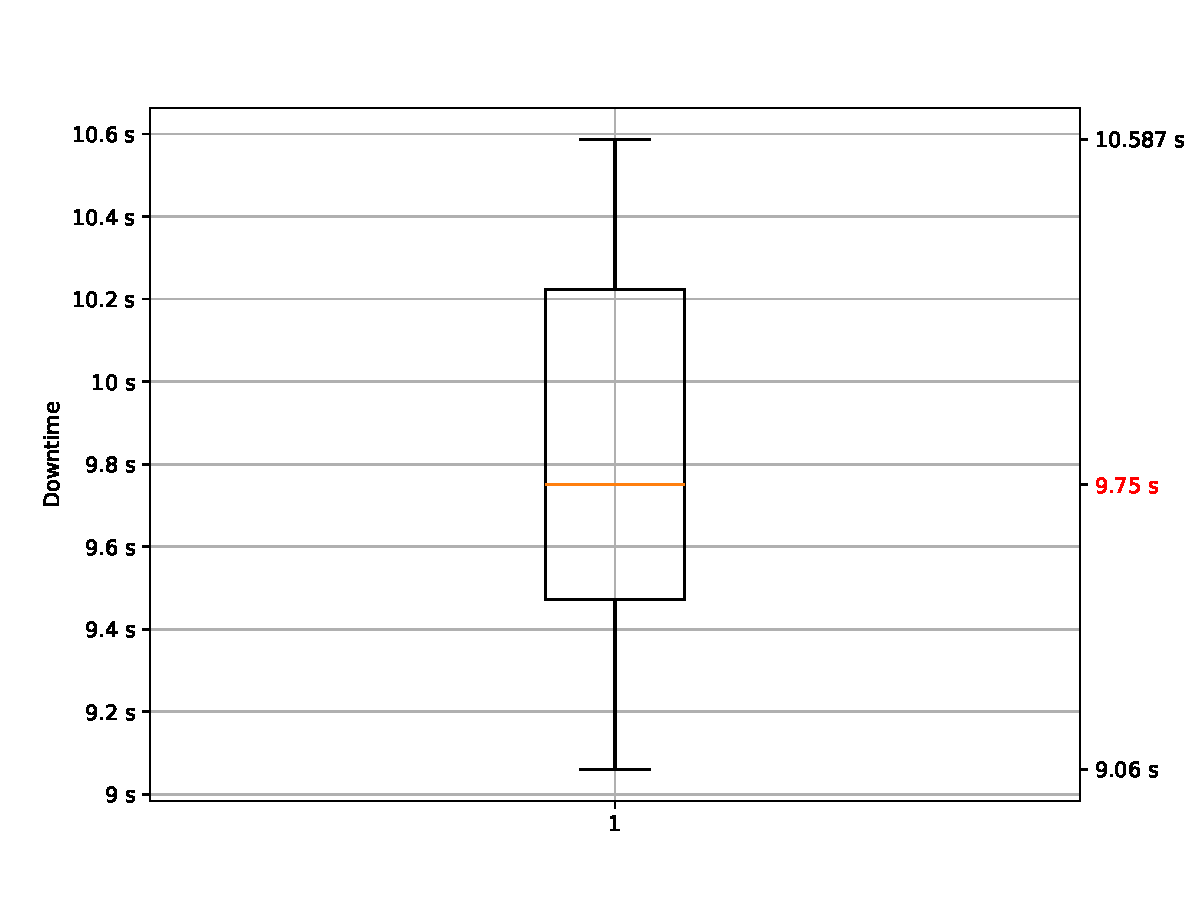
\includegraphics[scale=0.5]{Pictures/k3s-reaction}
\caption{Reaction to set virtual node as Not Ready in case of remote cluster disconnession}\label{graph:k-reaction}
\end{figure}

Moreover, using the same machines but connecting them through a single Kubernetes server and utilizing identical parameter settings, it was observed that the cluster response time in the event of a node failure is slightly higher by a few seconds compared to the time required to detect a node failure representing a Liqo cluster, as depicted in Figure~\ref{graph:k-reaction2}. This difference stems from the Virtual Kubelet's unique management and health check optimization implemented by Liqo, which supersedes traditional kubelet functions for the virtual node management.

\begin{figure}[ht]\centering
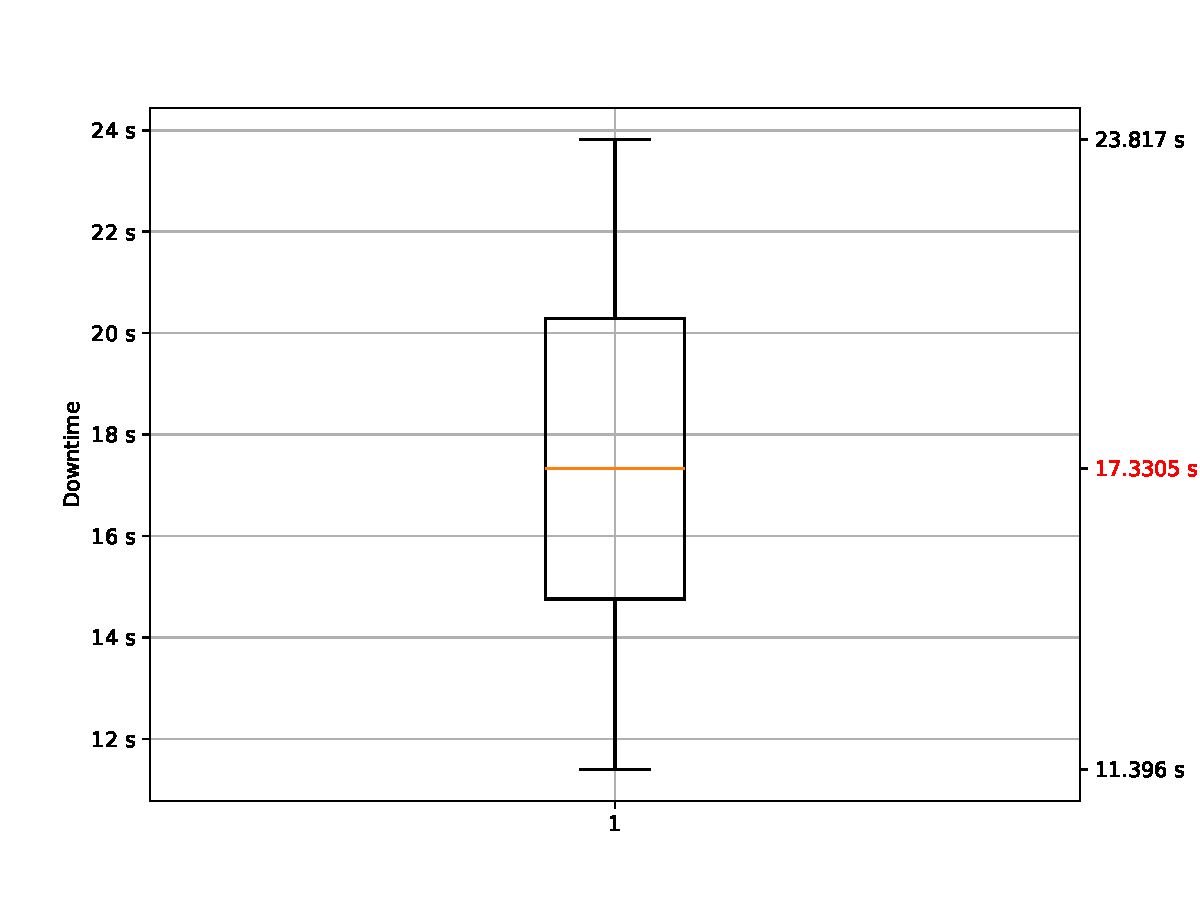
\includegraphics[scale=0.5]{Pictures/k3s-reaction2}
\caption{Reaction to set virtual node as Not Ready in case of local node disconnession}\label{graph:k-reaction2}
\end{figure}

\section{Stream reaction time}
The following tests demonstrate the downtime of a data stream from a PMU in the following scenarios:

\begin{enumerate}
\item Internal failure of a PDC pod, resulting in the rescheduling of the application. 
\item Fault/disconnection of the cluster hosting a PDC pod, resulting in the application being rescheduled to another cluster.
\end{enumerate}

Downtime is calculated from the timestamp of the last data frame of the old stream to the timestamp of the first data frame of the new stream, encompassing the time required for rescheduling the PDC pod, retrieving configurations from the database system, and reconnecting to the data stream.

These tests examine a data stream originating from a PMU that traverses through two PDC pod, one considered low-level and the other considered high-level, before reaching its intended application.

The use of the data frame timestamp is crucial due to the PMU's real-time production of data frames at 33-millisecond intervals, ensuring precise downtime calculations and analysis.

\subsection{Pod failure}
The failure scenario of the PDC pod was simulated by customizing the liveness probe mechanism, intentionally triggering a failure check after the pod had been running for 60 seconds. The pod was located in a remote cluster managed by Liqo.

The test results, displayed in Graph~\ref{graph:pod-down}, illustrate the median duration required for the lower-level PDC application to resume normal operation. This duration encompasses the time from detecting the PDC pod failure to its subsequent recovery, including the processes of restarting the pod, retrieving configurations from the system database, and re-establishing connection to the data stream.

Comparing these results with findings from previous thesis~\cite{e3-1} about the local solution using only Kubernetes,  where the pod recovery time ranged between 17-25 seconds, it is noted that here too, despite slight differences of a few seconds primarily due to environmental variables such as machine power, the order of magnitude remains consistent. 

\begin{figure}[ht]\centering
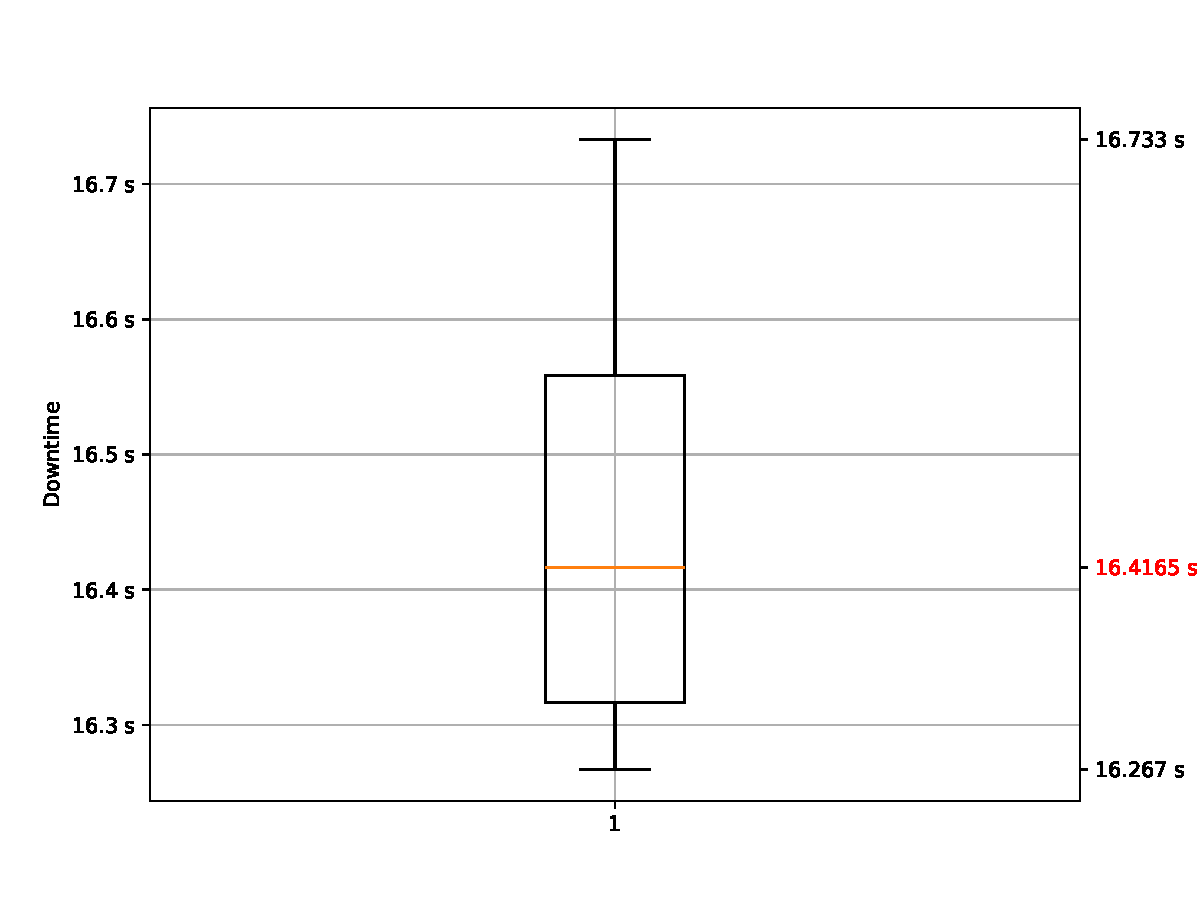
\includegraphics[scale=0.5]{Pictures/pdc-pod-down}
\caption{Box plot regarding stream downtime from last old data to the first new data in case of pod failure}\label{graph:pod-down}
\end{figure}

\subsection{Cluster failure}
The failure scenario was simulated by deliberately disabling the network interface of the lower-level PDC pod within the cluster. The deployment configuration of the lower-level PDC includes specific affinities to ensure that in the event of rescheduling, it can only be placed on another leaf cluster. As depicted in Figure~\ref{fig:test}, these leaf clusters are also managed by Liqo.

\begin{figure}[ht]\centering
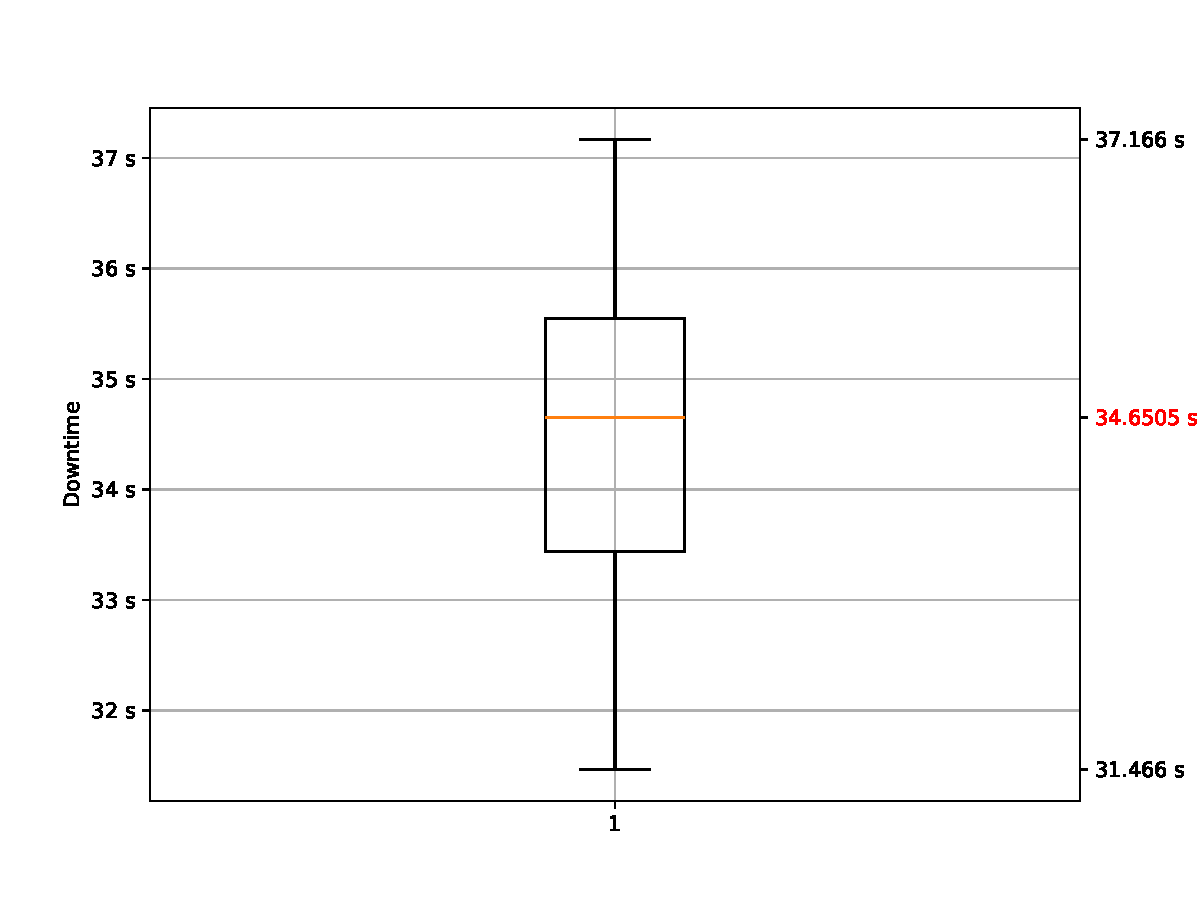
\includegraphics[scale=0.4]{Pictures/pdc-cluster-down}
\caption{Box plot regarding stream downtime from last old data to the first new data in case of cluster failure}\label{graph:cluster-down}
\end{figure}

The test results, displayed in Graph~\ref{graph:cluster-down}, illustrate the median duration required for the lower-level PDC application to resume normal operation. This duration includes the time required for the cluster to detect that the virtual node hosting the PDC is unreachable (9.75 seconds as shown in Graph~\ref{graph:k-reaction}), the waiting time before it can be rescheduled to another node (5 seconds as indicated in table \ref{t:1}), and the time necessary for the pod to restart (16.41 seconds as depicted in Graph~\ref{graph:pod-down}).

Comparing the results with the values shown in Figure ~\ref{fig:seba}, illustrating findings from the previous thesis~\cite{e3-1} focusing on the local solution using only Kubernetes, it is observed that the order of magnitude remains consistent. This reaffirms alongside previous tests that the introduction of Liqo technology does not introduce significant changes in terms of architectural overhead. In fact, in some cases, such as the optimization of the Kubelet, it enables better performance compared to the traditional Kubernetes architecture.


\begin{figure}[ht]\centering
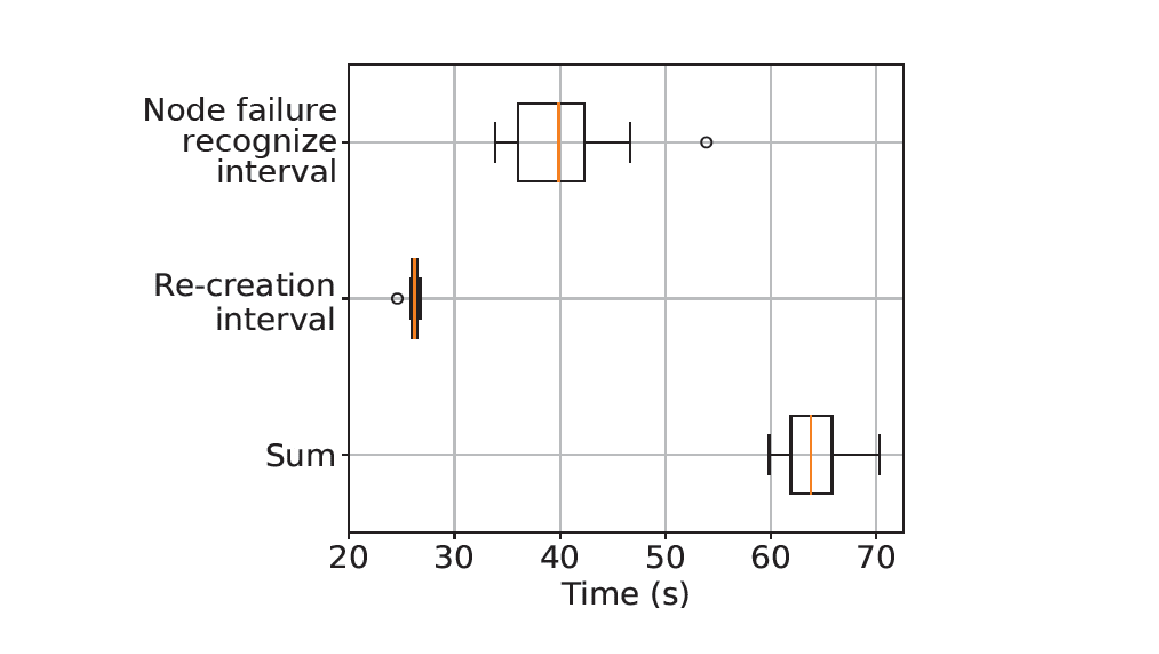
\includegraphics[scale=0.5]{Pictures/seba}
\caption{Time required to recover services on a disconnected node, on a traditional kubernetes cluster}\label{fig:seba}
\end{figure}

\section{Overall evaluation}
In this section, we summarize the findings from the various tests conducted to evaluate the performance, reliability, and resilience of the logical domain grouping implementation using Crownlabs and Liqo technology. The following points encapsulate the overall evaluation:

\begin{itemize}
\item \textbf{Test Environment and Configuration:} The test environment, meticulously configured using Crownlabs and Kubernetes clusters, accurately simulated real-world scenarios. The use of low-capacity virtual machines reflects typical setups in energy monitoring and distribution stations, ensuring relevance and applicability of the results. The fully-meshed star topology with a central root cluster efficiently managed the workload distribution and ensured robustness in case of node or cluster failures. The unidirectional peering for distributed database operations, as implemented through Liqo, facilitated seamless resource sharing and enhanced system reliability.

\item \textbf{Latency Analysis:} The latency tests revealed that the additional overhead introduced by Liqo technology is minimal. The measured average Liqo latency of 0.458 ms is well within acceptable limits for state estimation applications, which tolerate up to 1000 ms. This demonstrates that Liqo can be effectively utilized in distributed systems without significantly impacting communication performance.

\item \textbf{K3s Node Reaction Time:} The reaction time tests indicated that the introduction of Liqo technology did not introduce substantial delays. In fact, the Liqo-managed virtual kubelet demonstrated optimized health checks and node management, resulting in slightly faster response times in certain failure scenarios compared to traditional Kubernetes setups.

\item \textbf{Stream Reaction Time:} The tests simulating pod and cluster failures demonstrated that the downtime for resuming data streams was comparable to, if not slightly better than (in the case of cluster failure), traditional Kubernetes-only environments. This, along with new features such as the temporary independent management of a part of the network (with the continuation of the data stream inside) and the optimization of control capacity by a central entity to manage the rescheduling of the aggregator on other clusters, illustrates the significant advantages of introducing Liqo technology.

\item \textbf{Reliability and Resilience:} Overall, the tests conducted on the logical domain grouping architecture have demonstrated its high resilience against both internal and external cluster failures. Throughout the testing process, there was not a single instance where the system failed to automatically converge to a new stable state after a fault was introduced. Moreover, in scenarios where a cluster became disconnected, the system reliably reintegrated the cluster into the architecture automatically once the connection was restored. This seamless reintegration highlights the robustness and efficiency of the architecture in maintaining operational continuity and stability, underscoring the significant advantages of adopting this approach.

\item \textbf{Scalability and Flexibility:} The modular setup of clusters and the dynamic nature of Liqo peering allow for a high degree of adaptability, enabling the inclusion or exclusion of clusters without compromising the entire architecture. This is crucial for evolving system requirements and expanding infrastructure without significant overhauls. Scalability remains anchored to the official limits present in the Kubernetes documentation, although it has increased considerably since the set of nodes within a cluster is perceived as a single virtual node.

\item \textbf{Comparison with Traditional Kubernetes:} Throughout the evaluations, it was evident that the logical domain grouping implementation leveraging Liqo provided performance metrics on par with those of traditional Kubernetes architectures. Additionally, the introduction of Liqo offers several benefits, such as isolated operation in case of disconnections, enhanced central control over the entire network, and the ability to manage cluster failures that a Kubernetes-only architecture cannot easily implement.
\end{itemize}

In conclusion, the analyses confirm that the chosen implementation of logical domain grouping  offers a robust, scalable, and efficient solution for managing distributed systems. The minimal overhead introduced by Liqo, coupled with its advanced features, makes it a valuable addition to Kubernetes-based infrastructures, ensuring high resilience and optimal performance.


\chapter{Conclusion and future work}
The introduction of Liqo technology in research to implement the paradigms of Edge and Fog computing within the Smart Grid model has not only increased scalability by condensing multiple nodes into a single virtual node but has also enabled the introduction of new functionalities that were previously difficult to implement.

For example, in case of disconnection from the central network, the two parts of the network can operate autonomously, with the capability to deploy new applications until reconnection with the central network (island-mode operation).

The topology humorously called the "winning" topology for real implementation is the partial mesh star topology. Despite not being a complex architecture, it meets all constraints, stemming from the transparent operation of non-multi-cluster native applications, such as distributed database systems, and from design constraints like seeking the lowest possible power consumption and high resilience.

These results were described in the previous chapter, comparing them with the baseline solution values and demonstrating their similarity, without significant latency increases despite increased complexity.

Obviously, this solution does not represent a panacea for all issues; for instance, it is still quite limited in terms of scalability. A potential research direction could be to further explore the possibility of introducing a higher hierarchical level, as demonstrated in the second implementation in Chapter 6, while striving to maintain the high level of reliability demonstrated in this thesis.

This work was conducted using versions utilized in previous research to compare results and demonstrate the efficiency that Liqo technology enables. From this point, implementations on new versions could be developed, which provide access to new functionalities that could optimize the entire structure.

For example, the new versions of k3s and Percona allow the use of the spread operator, which would reduce the complexity of creating the logical hierarchical infrastructure.

Other future researches could focus on investigating the security implications of deploying such decentralized systems. Moreover, collaboration with industry partners could facilitate the transition from theoretical research to practical, real-world applications.

In conclusion, this thesis has demonstrated that integrating Liqo technology into Smart Grid models significantly enhances scalability and functionality. While challenges remain, the groundwork laid here provides a solid foundation for future advancements. The continued evolution and optimization of these technologies promise to drive significant improvements in the efficiency and resilience of critical infrastructures.







%%%%%%%%%%%%%%%%%%%%%%%%%%%%%%%%%%%%%%%%%%%%%%%%
%%%%%%%%%%%%%%%%%%%%%%%%%%%%%%%%%%%%%%%%%%%%%%%%


\bibliography{references}



\end{document}

